%%%%%%%%%%%%%%%%%%%%%%%%%%%%%%%%%%%%%%%%%%%%%%%%%%%%%%%%%%%%%%%%%%%%%%%%%%%%%%%
%%
%%          $Id: Rulebook.tex 2014-12-12 balkce $
%%    author(s): RoboCupAtHome Technical Committee(s)
%%  description: introduction to RoboCupAtHome
%%
%%%%%%%%%%%%%%%%%%%%%%%%%%%%%%%%%%%%%%%%%%%%%%%%%%%%%%%%%%%%%%%%%%%%%%%%%%%%%%%
\documentclass[11pt, twoside, openright, a4paper, chapterprefix]{scrbook}
\usepackage[inner=2.5cm, outer=2.5cm, top=4cm, bottom=4cm]{geometry}

%%% PACKAGES %%%%%%%%%%%%%%%%%%%%%%%%%%%%%%%%%%%%%%%%%%%%%%%%%%%%%%%%%%%%%%%%%%
%%%%%%%%%%%%%%%%%%%%%%%%%%%%%%%%%%%%%%%%%%%%%%%%%%%%%%%%%%%%%%%%%%%%%%%%%%%%%%%
%%
%%          $Id: packages.tex 385 2013-02-12 21:53:10Z holz $
%%    author(s): RoboCupAtHome Technical Committee(s)
%%  description: List of packages for the RoboCupAtHome rulebook
%%
%%%%%%%%%%%%%%%%%%%%%%%%%%%%%%%%%%%%%%%%%%%%%%%%%%%%%%%%%%%%%%%%%%%%%%%%%%%%%%%
% \usepackage{soul}

\usepackage[utf8x]{inputenc}
\usepackage[english]{babel}
\usepackage{amsmath,amssymb,amsfonts}
% \usepackage[nice]{nicefrac}
\usepackage{siunitx}
\usepackage{graphicx}
\usepackage{multicol}
\usepackage{verbatim}
\usepackage{fancyhdr}

% \usepackage{color}
\usepackage{xcolor}
\usepackage{colortbl}
% \usepackage{epsfig}
\usepackage{makeidx} % This one causes scoresheets not to setle
% \usepackage{lscape}
% \usepackage{picinpar}

\usepackage{./styles/tweaklist}

\usepackage{enumerate}
\usepackage{paralist}
\usepackage{multirow}
\usepackage{hhline}
\usepackage{pgffor}
% \usepackage{array}

\usepackage{nameref}
\usepackage{varioref}
\usepackage{hyperref}
\usepackage[noabbrev,nameinlink]{cleveref}
\usepackage{tabularx}
\usepackage{xspace}
\usepackage{csquotes}
\usepackage[inline]{enumitem}

%\usepackage{times}
%\usepackage{helvet}
%\usepackage{courier}

% \usepackage{url}
\usepackage{caption}
% \usepackage{epstopdf}
\usepackage{subfig}
\usepackage{float}
\usepackage{wrapfig}
% \usepackage{xfrac}

% \usepackage[titletoc]{appendix}
% \usepackage{enumitem}
% \usepackage{mathtools}
% \usepackage{gensymb}

% Required by scoresheets
\usepackage{calc}
\usepackage{ifthen}
\usepackage{environ}
\usepackage{wasysym}
\usepackage{chngpage}

% Local Variables:
% TeX-master: "../Rulebook"
% End:

\input{./setup/config.tex}
\input{./setup/styling.tex}


%%% MACROS %%%%%%%%%%%%%%%%%%%%%%%%%%%%%%%%%%%%%%%%%%%%%%%%%%%%%%%%%%%%%%%%%%%%
\input{./setup/active_version.tex}
\graphicspath{{\YEAR/}{./images/}}
%%%%%%%%%%%%%%%%%%%%%%%%%%%%%%%%%%%%%%%%%%%%%%%%%%%%%%%%%%%%%%%%%%%%%%%%%%%%%%%
%%
%%          $Id: macros.tex 399 2013-02-14 20:24:02Z holz $
%%    author(s): RoboCupAtHome Technical Committee(s)
%%  description: Macros for the RoboCupAtHome rulebook
%%
%%%%%%%%%%%%%%%%%%%%%%%%%%%%%%%%%%%%%%%%%%%%%%%%%%%%%%%%%%%%%%%%%%%%%%%%%%%%%%%

%%%%%%%%%%%%%%%%%%%%%%%%%%%%%%%%%%%%%%%%%%%%%%%%%%%%%%%%%%%%%%%%%%%%
% Macros for generating score sheets for RoboCup@Home              %
% to be used in the rulebook or during the competition             %
%                                                                  %
% Author: Dirk Holz & David Gossow                                 %
% Modif : Mauricio Matamoros                                       %
% $Id: macros_score_sheets.tex 429 2013-04-30 10:09:55Z holz $     %
%%%%%%%%%%%%%%%%%%%%%%%%%%%%%%%%%%%%%%%%%%%%%%%%%%%%%%%%%%%%%%%%%%%%
% chktex-file 1
% chktex-file 15
% chktex-file 21
% chktex-file 35
% chktex-file 44

% %%% %%%%%%%%%%%%%%%%%%%%%%%%%%%%%%%%%%%%%%%%%%%%%%%%%%%%%%%%%%%%%%
%                                                                  %
% GLOBAL OPTIONS                                                   %
%                                                                  %
% %%% %%%%%%%%%%%%%%%%%%%%%%%%%%%%%%%%%%%%%%%%%%%%%%%%%%%%%%%%%%%%%%

% Set \shortScoresheet to true for the rulebook version
% Set \shortScoresheet to false for the referee's scoresheet
\newcommand{\shortScoresheet}{true}

% The global number of attempts per test
\newcommand{\attempts}{3}

% Sets the total penalty for not showing up
\newcommand{\notattendingpenalty}{500}

% Set to true to display the "Using start button" penalty item
\newcommand{\startbuttonpenalized}{true}

% Sets the total penalty for not using start button instead of door
\newcommand{\startbuttonpenalty}{100}

% Set to true to display the the outstanding performance bonus item
\newcommand{\outstandingPerformanceBonus}{true}

% Percentage of the outstanding performance bonus (ommit % symbol)
\newcommand{\outstandingPerformanceBonusPercentage}{10}

% Set to true to display the data recording bonus item
\newcommand{\dataRecordingBonus}{false}

% Percentage of the data recording bonus (ommit % symbol)
\newcommand{\dataRecordingBonusPercentage}{10}

% Sets the name of the column for referee scoring when \attempts=1
\newcommand{\singleTryColumnCaption}{Single try}

% Sets the first column's name for referee scoring when \attempts=2
\newcommand{\firstTryColumnCaption}{First try}

% Sets the second column's name for referee scoring when \attempts=2
\newcommand{\secondTryColumnCaption}{Restart}

% Sets the name of the column for referee scoring when \attempts=1
\newcommand{\firstColumnCaption}{Action}

% Sets the second column's name for referee scoring when \attempts=2
\newcommand{\secondColumnCaption}{Score}

% %%% %%%%%%%%%%%%%%%%%%%%%%%%%%%%%%%%%%%%%%%%%%%%%%%%%%%%%%%%%%%%%%
%                                                                  %
% USAGE                                                            %
%                                                                  %
% %%% %%%%%%%%%%%%%%%%%%%%%%%%%%%%%%%%%%%%%%%%%%%%%%%%%%%%%%%%%%%%%%
%
% A scoresheet must be in a separated tex file. Scoring marks are
% presented as a list within the {scorelist} environment. Each
% mark is enlisted using the \scoreitem macro. Headings can be
% defined with the \scoreheading macro. Within the scoresheet
% booklet the {scorelist} environment shall be placed inside the
% {scoresheet} environment that adds the footer and heading required
% by the referee.
%
% -= Snippet (rulebook.tex) =-
%     \newpage%
%     \input{my_score_sheet.tex}
% -= End Snippet =-
%
% -= Snippet (score_sheets.tex) =-
%     \begin[options]{scoresheet}
%     \input{my_score_sheet.tex}
%     \end{scoresheet}
% -= End Snippet =-
%
% -= Snippet (my_score_sheet.tex) =-
%     \begin[options]{scorelist}
%       \scoreheading{Main goal}
%       \scoreitem[multiplier]{score}{Description}
%       % These do not contribute to automatic scoring calculation
%       \scorebonus[multiplier]{score}{Description}
%       \scorepenalty[multiplier]{score}{Description}
%     \end{scorelist}
% -= End Snippet =-
%
%
% scorelist options:
% The scorelist environment supports the following comma-separated
% optional arguments:
%   - score              Integer. Sets the test total score to an
%                        arbitrary value (disables autocalc)
%   - attempts           Integer. Number of attempts for the
%                        scoresheet (default is \global\attempts)
%   - continue           Not implemented
%   - datarecording      Boolean. Toggles the "Data Recording"
%                        item under Special penalties and standard
%                        bonuses
%   - datarecordingpc    Integer. Percentage for the data
%                        recording bonus
%   - datarecordingbonus Integer. Arbitrary value for the data
%                        recording bonus
%   - outstanding        Boolean. Toggles the "Outstanding
%                        Performance" item under Special penalties
%                        and standard bonuses
%   - outstandingpc      Integer. Percentage for the
%                        outstanding performance bonus
%   - outstandingbonus   Integer. Arbitrary value for the
%                        outstanding performance bonus
%   - startbutton        Boolean. Toggles the "Using start button"
%                        item under Special penalties and standard
%                        bonuses.
%   - startbuttonpenalty Integer. Arbitrary value for the Using
%                        start button penalty.
%   - firstcolcaption    String. Caption for the first column of
%                        the scoresheet (default="Action")
%   - secondcolcaption   String. Caption for the second column of
%                        the scoresheet (default="Score")
%   - singletrycc        String. Caption of the first column for
%                        referee scoring when attempts=1
%   - firsttrycc         String. Caption of the first column for
%                        referee scoring when attempts=2
%   - secondtrycc        String. Caption of the second column for
%                        referee scoring when attempts=2
%
%
%
% scoreitem, scorebonus, and scorepenalty arguments
%   #1 multiplier   A number indicating how many times the mark
%                   can be scored. It is printed at the left of
%                   the score followed by the \times symbol.
%   #2 score        Scoring points. Printed at the right of the
%                   description
%   #3 description  A description for the score mark
%
%
%
%
%
%
%
%
%
%
%
%
%
%
%
%
%
%
%
%
%
%
%
%
%
%
%
%
%
%
%
%
%
%
%
%
%
%
%
%
%
%
%
%
%
%
%
%
%
%
% %%% %%%%%%%%%%%%%%%%%%%%%%%%%%%%%%%%%%%%%%%%%%%%%%%%%%%%%%%%%%%%%%
%                                                                  %
% FROM HERE ON, THERE IS NOTHING TO CHANGE                         %
%                                                                  %
% %%% %%%%%%%%%%%%%%%%%%%%%%%%%%%%%%%%%%%%%%%%%%%%%%%%%%%%%%%%%%%%%%

%%% Counters / temp. variables %%%%%%%%%%%%%%%%%
\newcounter{currTestScore}
\newcounter{currTestScoreTotal}
\newcounter{currTestScoreTotalWithoutBonus}
\newcounter{currOutstandingBonus}
\newcounter{currDataRecordingBonus}


% set \continueAvailable to true for CONTINUE sections
\newcommand{\continueAvailable}{true}


% name of the current test, is set automatically in the rulebook
\newcommand{\currentTest}{}

% (internal) if-clause shortcut to switch between short rulebook version and full score sheet for referees
\newcommand{\ifShortScoresheet}[2]{%
	\ifthenelse{ \equal{\shortScoresheet}{true} }{#1}{#2}%
}

% (internal) draws the scoresheet line for score handwritting
\newcommand{\scoreline}[1][0.08]{\rule{#1\linewidth}{.2pt}}

% (internal) returns absolute value of argument
\newcommand{\absval}[1]{\ifnum#1<0 -\fi#1}
















% %%% %%%%%%%%%%%%%%%%%%%%%%%%%%%%%%%%%%%%%%%%%%%%%%%%%%%%%%%%%%%%%%
%                                                                  %
% ENVIRONMENT: scoresheet                                          %
% Scoresheet page layout                                           %
%                                                                  %
% %%% %%%%%%%%%%%%%%%%%%%%%%%%%%%%%%%%%%%%%%%%%%%%%%%%%%%%%%%%%%%%%%

\newenvironment{scoresheet}{%
% \begin{scoresheet}
	\newpage%
	%
	% Test, team, and referee info
	%
	\begin{minipage}[t]{0.85\textwidth}%
		\vspace{0pt}%
		{\huge \textbf{Score Sheet} }%
		\vspace{2 em}%

		\begin{tabular}{ @{} l l l}
			\textbf{Test:} & \currentTest \\[.9 em]%
			\textbf{Team name:} & \scoreline[0.6]\\[.9 em]%
			\textbf{Referee name:} & \scoreline[0.6]\\[.9 em]%
		\end{tabular}%
		\vspace{0.5 em}%

	\end{minipage}
	\hfill
	%
	% @Home Logo
	%
	\begin{minipage}[t]{0.15\textwidth}%
		\vspace{0pt}%
		\includegraphics[width=\textwidth]{images/logo_RoboCupAtHome.jpg}%
	\end{minipage}\\%
}{
% \end{scoresheet}
	\vspace{0.5 em}%
	\textbf{Remarks:}%

	%
	% Signatures of referee / team leader %%%%%%%%%%%%
	%
	\vfill
	\begin{tabular*}{\linewidth}{@{} @{\extracolsep{\fill}} l l l @{}}
		\scoreline[0.25] \hspace{0.05\linewidth}%
			& \scoreline[0.25] \hspace{0.05\linewidth}%
			& \scoreline[0.25]%
		\\
		\textit{Date \& time}%
			& \textit{Referee} %
			& \textit{Team leader}%
	\end{tabular*}

	\newpage
}














% %%% %%%%%%%%%%%%%%%%%%%%%%%%%%%%%%%%%%%%%%%%%%%%%%%%%%%%%%%%%%%%%%
%                                                                  %
% ENVIRONMENT: scorelist                                           %
% Score list table                                                 %
%                                                                  %
% %%% %%%%%%%%%%%%%%%%%%%%%%%%%%%%%%%%%%%%%%%%%%%%%%%%%%%%%%%%%%%%%%

\usepackage{pgfkeys}
\pgfkeys{
	/scorelist/.is family, /scorelist,
	default/.style={
		attempts = \attempts,
		continue = true,
		datarecording = \dataRecordingBonus,
		datarecordingpc = \dataRecordingBonusPercentage,
		datarecordingbonus = 0,
		outstanding = \outstandingPerformanceBonus,
		outstandingpc = \outstandingPerformanceBonusPercentage,
		outstandingbonus = 0,
		startbutton = \startbuttonpenalized,
		startbuttonpenalty = \startbuttonpenalty,
		firstcolcaption = \firstColumnCaption,
		secondcolcaption = \secondColumnCaption,
		singletrycc = \singleTryColumnCaption,
		firsttrycc = \firstTryColumnCaption,
		secondtrycc = \secondTryColumnCaption,
	},
	attempts/.estore in = \scorelistAttempts,
	continue/.estore in = \scorelistContinue,
	datarecording/.estore in = \scorelistDataRecording,
	datarecordingpc/.estore in = \scorelistDataRecordingPercentage,
	datarecordingbonus/.estore in = \scorelistDataRecordingBonus,
	outstanding/.estore in = \scorelistOutstanding,
	outstandingpc/.estore in = \scorelistOutstandingPercentage,
	outstandingbonus/.estore in = \scorelistOutstandingBonus,
	startbutton/.estore in = \scorelistStartButton,
	startbuttonpenalty/.estore in = \scorelistStartButtonPenalty,
	firstcolcaption/.estore in = \scorelistFirstColCaption,
	secondcolcaption/.estore in = \scorelistSecondColCaption,
	singletrycc/.estore in = \scorelistSingleTryCC,
	firsttrycc/.estore in = \scorelistFirstTryCC,
	secondtrycc/.estore in = \scorelistSecondTryCC,
}

\makeatletter%
\NewEnviron{scorelist}[1][]{
% \begin{scorelist}
	%%%%%%%%%%%%%%%%%%%%%%%%%%%%%%%%%%%%%%%%%%%%%%%%%%%%%%%%%%%%%%%
	% read options
	%%%%%%%%%%%%%%%%%%%%%%%%%%%%%%%%%%%%%%%%%%%%%%%%%%%%%%%%%%%%%%%
	\pgfkeys{/scorelist, default, #1}%

	%%%%%%%%%%%%%%%%%%%%%%%%%%%%%%%%%%%%%%%%%%%%%%%%%%%%%%%%%%%%%%%
	% init variables %%%%%%%%%%%%%%%%%%%%%%%%%%%%%%%%%%%%%%%%%%%%%%
	%%%%%%%%%%%%%%%%%%%%%%%%%%%%%%%%%%%%%%%%%%%%%%%%%%%%%%%%%%%%%%%
	\setcounter{currTestScore}{0}
	\setcounter{currOutstandingBonus}{\scorelistOutstandingBonus}
	\setcounter{currDataRecordingBonus}{\scorelistDataRecordingBonus}

	%%%%%%%%%%%%%%%%%%%%%%%%%%%%%%%%%%%%%%%%%%%%%%%%%%%%%%%%%%%%%%%
	% environment commands %%%%%%%%%%%%%%%%%%%%%%%%%%%%%%%%%%%%%%%%
	%%%%%%%%%%%%%%%%%%%%%%%%%%%%%%%%%%%%%%%%%%%%%%%%%%%%%%%%%%%%%%%

	% heading %%%%%%%%%%%%%%%%%%%%%%%%%%%%%%%%%%%%%%%%%%%%%%%%%%%%%
	\newcommand{\scoreheading}[1]{%
		\ifShortScoresheet{%
			\xdef\@scoreheadingcolspan{2}%
		}{%
			\xdef\@scoreheadingcolspan{\the\numexpr2+\scorelistAttempts\relax}%
		}%
		\phantom{.} \\[-12pt]%
		\multicolumn{\@scoreheadingcolspan}{@{}l}{\textbi{##1}}\\[0pt]%
	}

	\newcommand{\scoreitem}[3][1]{%
		\ifthenelse{ ##2 > 0 }{%
			\addtocounter{currTestScore}{ ##2 * ##1 }%
		}{}%
		%
		\@scoreitem[##1]{##2}{##3}%
	}

	\newcommand{\penaltyitem}[3][1]{%
		\ifthenelse{##2 < 0}{%
			\@scoreitem[##1]{\absval{##2}}{##3}%
		}{%
			\@scoreitem[##1]{\absval{-##2}}{##3}%
		}%
	}

	\newcommand{\bonusitem}[3][1]{%
		\@scoreitem[##1]{##2}{##3}%
	}

	% Alias of \bonusitem
	\newcommand{\scorebonus}[3][1]{\bonusitem[##1][##2][##3]}

	% Alias of \penaltyitem
	\newcommand{\scorepenalty}[3][1]{\penaltyitem[##1][##2][##3]}

	%%%%%%%%%%%%%%%%%%%%%%%%%%%%%%%%%%%%%%%%%%%%%%%%%%%%%%%%%%%%%%%
	% Commands for overriding internal calculations %%%%%%%%%%%%%%%
	%%%%%%%%%%%%%%%%%%%%%%%%%%%%%%%%%%%%%%%%%%%%%%%%%%%%%%%%%%%%%%%

	% set score counter to arbitrary value %%%%%%%%%%%%%%%%%%%%%%%%
	\newcommand{\setTotalScore}[1]%
	{%
		\setcounter{currTestScore}{##1}%
	}

	% set outstanding bonus counter to arbitrary value %%%%%%%%%%%%
	\newcommand{\setOutstandingBonus}[1]%
	{%
		\setcounter{currOutstandingBonus}{##1}%
	}

	%%%%%%%%%%%%%%%%%%%%%%%%%%%%%%%%%%%%%%%%%%%%%%%%%%%%%%%%%%%%%%%
	% environment internal commands %%%%%%%%%%%%%%%%%%%%%%%%%%%%%%%
	%%%%%%%%%%%%%%%%%%%%%%%%%%%%%%%%%%%%%%%%%%%%%%%%%%%%%%%%%%%%%%%

	% table entry %%%%%%%%%%%%%%%%%%%%%%%%%%%%%%%%%%%%%%%%%%%%%%%%%
	\newcommand{\@scoreitem}[3][1]{%
		##3\vspace{0.1em} &%
		\textit{%
			\ifthenelse{ \equal{##2}{0} }{~}{% else
				\ifthenelse{ \equal{##1}{1} }{}{##1$\times$}%
			##2}%
		}%
		\ifShortScoresheet{}{&\attemptScoreLines{\scorelistAttempts}}\\[0pt]%
	}

	% [INTERNAL] writes down the line for the final total score %%%
	\newcommand{\scoreTotal}{%
		\\%
		\textbf{Total score~}%
		\ifShortScoresheet{%
			(excluding penalties and standard bonuses) &%
			\textit{\thecurrTestScoreTotalWithoutBonus}%
		}{%
			&\textit{\thecurrTestScoreTotal}
			&\multicolumn{\scorelistAttempts}{c}{\scoreline[0.20]}%
		}\\[0pt]%
	}

	% [INTERNAL] writes down the lines for the total score per try
	\newcommand{\scorePerTry}{%
		\\%
		\ifShortScoresheet{}{%
			\ifthenelse{ \attempts > 1 }{%
				\textbi{Score per try} &%
				\textit{\thecurrTestScoreTotalWithoutBonus} &%
				\attemptScoreLines{\scorelistAttempts}%
				\\[0pt]%
			}{}%
		}%
	}

	% [INTERNAL] draws a line for referee scoring %%%%%%%%%%%%%%%%%
	\gdef\@marklinewidth{0.06}
	\newcommand{\markline}{\rule{\@marklinewidth\linewidth}{.2pt}}

	% [INTERNAL] draws all the line for referee scoring %%%%%%%%%%%
	\newcommand{\attemptScoreLines}[1]{%
		\protected@xdef\@scorelines{\markline}%
		\ifthenelse{##1 > 1}{%
			\foreach \i in {2,...,##1}{%
				\protected@xdef\@scorelines{\@scorelines & \markline}%
			}%
		}{}%
		\@scorelines%
	}

	% [INTERNAL] writes down the headings for referee scoring %%%%%
	\newcommand{\attemptHeadings}[1]{%
		\ifthenelse{\equal{##1}{1}}{%
			\gdef\@attemptheadings{\textbf{\scorelistSingleTryCC}}%
			\gdef\@marklinewidth{0.1}%
		}{}%
		\ifthenelse{\equal{##1}{2}}{%
			\gdef\@attemptheadings{\textbf{\scorelistFirstTryCC} & \textbf{\scorelistSecondTryCC}}%
			\gdef\@marklinewidth{0.08}%
		}{}%
		\ifthenelse{##1 > 2}{
			\protected@xdef\@attemptheadings{%
				\textbf{\small$1^{st}$~try} &%
				\textbf{\small$2^{nd}$~try} &%
				\textbf{\small$3^{rd}$~try}}%
		}{}%
		\ifthenelse{##1 > 3}{
			\foreach \i in {4,...,##1}{% chktex11
				\protected@xdef\@attemptheadings{%
					\@attemptheadings &%
					\textbf{\small$\i^{th}$~try}%
				}%
			}%
			\gdef\@marklinewidth{0.06}%
		}{}%
		\@attemptheadings%
	}

	%%%%%%%%%%%%%%%%%%%%%%%%%%%%%%%%%%%%%%%%%%%%%%%%%%%%%%%%%%%%%%%
	% setup table %%%%%%%%%%%%%%%%%%%%%%%%%%%%%%%%%%%%%%%%%%%%%%%%%
	%%%%%%%%%%%%%%%%%%%%%%%%%%%%%%%%%%%%%%%%%%%%%%%%%%%%%%%%%%%%%%%
	\vspace{0.8 em}%
	\noindent%
	\begin{tabularx}{\textwidth}{ @{}X @{}r *{\scorelistAttempts}{c}}
		\textbf{\scorelistFirstColCaption} &%
		\textbf{\scorelistSecondColCaption}%
		\ifShortScoresheet{}{&\attemptHeadings{\scorelistAttempts}}
	\\\hline



\BODY



	%%%%%%%%%%%%%%%%%%%%%%%%%%%%%%%%%%%%%%%%%%%%%%%%%%%%%%%%%%%%%%%
	% calculate max. score, and bonuses %%%%%%%%%%%%%%%%%%%%%%%%%%%
	%%%%%%%%%%%%%%%%%%%%%%%%%%%%%%%%%%%%%%%%%%%%%%%%%%%%%%%%%%%%%%%
	% base total score (accumulative) %%%%%%%%%%%%%%%%%%%%%%%%%%%%%
	\setcounter{currTestScoreTotal}{\thecurrTestScore}
	% outstanding performance bonus %%%%%%%%%%%%%%%%%%%%%%%%%%%%%%%
	\ifthenelse{\equal{\scorelistOutstanding}{true}}{%
		\ifthenelse{ \equal{\thecurrOutstandingBonus}{0} }{%
			\setcounter{currOutstandingBonus}{ \thecurrTestScore*\scorelistOutstandingPercentage/100 }
		}{}%
		\setcounter{currTestScoreTotal}{%
			\thecurrTestScoreTotal + \thecurrOutstandingBonus}%
	}{}%
	% data recording bonus %%%%%%%%%%%%%%%%%%%%%%%%%%%%%%%%%%%%%%%%
	\ifthenelse{\equal{\scorelistDataRecording}{true}}{%
		\ifthenelse{ \equal{\thecurrDataRecordingBonus}{0} }{%
			\setcounter{currDataRecordingBonus}{ \thecurrTestScore*\scorelistDataRecordingPercentage/100 }%
		}{}%
		\setcounter{currTestScoreTotal}{%
			\thecurrTestScoreTotal + \thecurrOutstandingBonus}%
	}{}%
	\setcounter{currTestScoreTotalWithoutBonus}{ \thecurrTestScore }

	%%%%%%%%%%%%%%%%%%%%%%%%%%%%%%%%%%%%%%%%%%%%%%%%%%%%%%%%%%%%%%%
	% Special penalties & bonuses %%%%%%%%%%%%%%%%%%%%%%%%%%%%%%%%%
	%%%%%%%%%%%%%%%%%%%%%%%%%%%%%%%%%%%%%%%%%%%%%%%%%%%%%%%%%%%%%%%
	\scoreheading{Special penalties \& standard bonuses}

	% not showing up penalty %%%%%%%%%%%%%%%%%%%%%%%%%%%%%%%%%%%%%%
	\penaltyitem{\notattendingpenalty}{Not attending \ifShortScoresheet{(see sec.~\ref{rule:not_attending})}{}}

	% require signal for door opening %%%%%%%%%%%%%%%%%%%%%%%%%%%%%
	\ifthenelse{ \equal{\scorelistStartButton}{true} }{
	  \penaltyitem{\scorelistStartButtonPenalty}{Using start button \ifShortScoresheet{(see sec.~\ref{rule:start_button})}{}}
	}{}

	% data recording bonus %%%%%%%%%%%%%%%%%%%%%%%%%%%%%%%%%%%%%%%%
	\ifthenelse{%
		\thecurrDataRecordingBonus>0 \AND %
		\equal{\scorelistDataRecording}{true}%
	}{%
		\bonusitem{\thecurrDataRecordingBonus}{Contributing with recorded data ($\frac{\sum gathered~points}{max~points} \times$) \ifShortScoresheet{(see sec.~\ref{rule:datarecording})}{}}%
	}{}%

	% outstanding performance bonus %%%%%%%%%%%%%%%%%%%%%%%%%%%%%%%
	\ifthenelse{%
		\value{currOutstandingBonus}>0 \AND %
		\equal{\scorelistOutstanding}{true}%
	}{%
		\bonusitem{\thecurrOutstandingBonus}{Outstanding performance~\ifShortScoresheet{(see sec.~\ref{rule:outstanding_performance})}{}}%
	}{}%
	%
	% Total score %%%%%%%%%%%%%%%%%%%%%%%%%%%%%%%%%%%%%%%%%%%%%%%%%
	\\[-1em]\hline
	\scorePerTry
	\scoreTotal

	\end{tabularx}
}
\makeatother%

% Local Variables:
% TeX-master: "../Rulebook"
% End:
%

\input{./setup/macros_open_demonstrations.tex}
\input{./setup/macros_leagues.tex}

\newcommand{\rulebookVersion}{\STATE\ version for RoboCup \YEAR\xspace(\VERSION)}

\def\RoboCup{{\textsc{RoboCup}}}
\def\Robocup{{\textsc{RoboCup}}}
\def\robocup{{\textsc{RoboCup}}}
\def\AtHome{{\textsc{RoboCup@Home}}}
\def\MSL{\textsc{Middle Size League}}
\def\MS{{\textsc{Middle Size}}}
\def\SSL{\textsc{Soccer Simulation League}}
\def\SS{\textsc{Soccer Simulation}}

\def\TC{technical committee (TC)}
\def\OC{organizing committee (OC)}

\newcommand{\textbi}[1]{\textbf{\textit{#1}}}
\renewcommand{\labelenumi}{\arabic{enumi}.}
\renewcommand{\labelenumii}{\labelenumi\arabic{enumii}.}
\renewcommand{\labelenumiii}{\labelenumii.\arabic{enumiii}.}

\newcommand{\testtocentry}[1]{%
	\nameref{#1}\dotfill\pageref{#1}\\[0.2\baselineskip]%
}

%% %%%%%%%%%%%%%%%%%%%%%%%%%%%%%%%%%%%%%%%%%%%%%%%%%%%%%%%%% %%
%%                    Developement-Tools                     %%
%% %%%%%%%%%%%%%%%%%%%%%%%%%%%%%%%%%%%%%%%%%%%%%%%%%%%%%%%%% %%

%% %%%%%%%%%%%%%%%%%%%%%%%%%%%%%%%%%%%%%%%
\newcommand{\tbc}[1]{\textbf{\it\color{red}{t.b.c. ...}#1\color{black}}}
\newcommand{\todo}[1]{\textbf{\it\color{red}{todo: }#1\color{black}}}
\newcommand{\TODO}[1]{\textbf{\it\color{red}{TODO:\\}#1\color{black}}}
\newcommand{\chk}[1]{\textbf{\color{red}#1\color{black}}}

\newcommand{\reworkon}{\marginpar{\raggedright\color{red}{$\downarrow$rework}\color{black}}}
\newcommand{\reworkoff}{\marginpar{\raggedright\color{red}{$\uparrow$rework}\color{black}}}

%% %%%%%%%%%%%%%%%%%%%%%%%%%%%%%%%%%%%%%%%
%%  site notes/margin notes
\def\note#1{\marginpar{\raggedright\tiny#1}}
\def\mpar#1{\marginpar{\raggedright\tiny#1}}
\def\rand#1{\marginpar{\raggedright\tiny#1}}
\setlength{\marginparwidth}{2cm}

\newcommand{\refsec}[1]{Section~\ref{#1}}
\newcommand{\reftab}[1]{Table~\ref{#1}}
\newcommand{\reffig}[1]{Figure~\ref{#1}}

%% %%%%%%%%%%%%%%%%%%%%%%%%%%%%%%%%%%%%%%%
%% side-annotation-macros for easy lookup
% \newcommand{\awardmark}{\marginpar{\centering\includegraphics[width=.34cm]{images/icon_award.pdf}}}
% \newcommand{\refmark}{\marginpar{\centering\includegraphics[width=.5cm]{images/icon_whistle.pdf}}}
% \newcommand{\referee}[1]{\emph{#1}\marginpar{\centering\includegraphics[width=.5cm]{images/icon_whistle.pdf}}}
% \newcommand{\scoremark}{\marginpar{\centering\includegraphics[width=.34cm]{images/icon_score.pdf}}}
\newcommand{\awardmark}{}
\newcommand{\refmark}{}
\newcommand{\referee}[1]{}
\newcommand{\scoremark}{}
%\newcommand{\scoring}[1]{\emph{#1}\marginpar{\centering\includegraphics[width=.34cm]{images/icon_score.pdf}}}
\newcommand{\scoring}[1]{\emph{#1}}
\newcommand{\timark}{\marginpar{\centering\includegraphics[width=.34cm]{icon_clock.pdf}}}

%\newcommand{\timing}[1]{\emph{#1}\marginpar{\centering\includegraphics[width=.34cm]{images/icon_clock.pdf}}}
\newcommand{\timing}[1]{\emph{#1}}

\def\svnRevision{Unknown} %
\def\svnChangeData{Unknown} %
\def\revnumtmpfile{.temp_ruleook_version}
\def\revdattmpfile{.temp_ruleook_date}
\immediate\write18{git rev-list HEAD | wc -l > \revnumtmpfile}
%\immediate\write18{svnversion . > \revnumtmpfile}
\IfFileExists{\revnumtmpfile}{\def\svnRevision{\input{\revnumtmpfile}\unskip}}{}
\immediate\write18{git log -1 --date=short  | grep 'Date:' | awk '{print $2}'> \revdattmpfile}
%\immediate\write18{svn info | grep 'Last Changed Date:' | awk '{print $4}'> \revdattmpfile}
\IfFileExists{\revdattmpfile}{\def\svnChangeData{\input{\revdattmpfile}\unskip}}{}
% \IfFileExists{\revnumtmpfile}{\immediate\write18{rm -f \revnumtmpfile}}{}
% \IfFileExists{\revdattmpfile}{\immediate\write18{rm -f \revdattmpfile}}{}
\newcommand{\VERSION}{Revision \svnChangeData\_\svnRevision}


% Local Variables:
% TeX-master: "../Rulebook"
% End:

\input{./setup/abbrevix.tex}



\makeindex                                % generate index
\makeabbex                                % generate abbreviations





%\newcommand{\sectionbreak}{\clearpage}
%\newcommand{\subsectionbreak}{\clearpage}


\begin{document}

\input{./pages/titlepage}

\pagestyle{empty}
%% %%%%%%%%%%%%%%%%%%%%%%%%%%%%%%%%%%%%%%%%%%%%%%%%%%%%%%%%%%%%%%%%%%%%%%%%%%%
%%
%%          $Id: acknowledgments.tex 404 2013-02-15 08:51:20Z sugiura $
%%    author(s): RoboCupAtHome Technical Committee(s)
%%  description: Acknowledgments for the RoboCupAtHome RuleBook
%%
%% %%%%%%%%%%%%%%%%%%%%%%%%%%%%%%%%%%%%%%%%%%%%%%%%%%%%%%%%%%%%%%%%%%%%%%%%%%%



\section*{About This Rulebook}
This is the official rulebook of the \YEAR ~RoboCup@Home competition.
It has been written by the \YEAR ~RoboCup@Home Technical Committee with the special collaboration of (in alphabetical order):
% Mauricio Matamoros,
% and
% Loy van Beek.



\section*{How to Cite This Rulebook}
If you refer to RoboCup@Home and this rulebook in particular, please cite:

Mauricio Matamoros, Caleb Rascon, Justin Hart, Dirk Holz, Kai Chen, and Loy van Beek.
\enquote{Robocup@Home \YEAR: Rule and regulations,}
\url{http://www.robocupathome.org/rules/2019_rulebook.pdf}, \YEAR.

\begin{center}
\begin{minipage}{0.8\textwidth}
	\footnotesize%
	\verbatiminput{citation.bib}
\end{minipage}
\end{center}

\section*{Acknowledgments}
\label{sec:acknowledgments}
We would like to thank the members of the Technical Committee who put up the rules and the Organizing Committee who organizes the competition.

~\\\noindent People that have been working on this rulebook as member of one of the league's committees (in alphabetical order):
\begin{center}
\begin{minipage}{0.8\textwidth}
\begin{multicols}{3}%
\footnotesize
\noindent%

% Kai Chen\\
% Justin Hart\\
% Luca Iocchi\\
% Mauricio Matamoros\\
% Dirk Holz\\
% \columnbreak
% Raphael Memmesheimer\\
% Alexander Moriarty\\
% Caleb Rascon\\
% Sammy Pfeiffer\\
% \columnbreak
% Komei Sugiura\\
% Sven Wachsmuth\\
% Tijn van der Zant\\
\end{multicols}
\end{minipage}
\end{center}

We also like to thank all the people who contributed to the RoboCup@Home league with their feedback and comments.

~\\\noindent People that have been working on this rulebook as member the league (in alphabetical order):
\begin{center}
\begin{minipage}{0.8\textwidth}
\begin{multicols}{2}%
\footnotesize
\noindent%
% Loy van Beek (@LoyVanBeek)\\
% Sebastian Meyer zu Borgsen (@semeyerz)\\
% Matthijs van der Burgh (@MatthijsBurgh)\\
% Remi Fabre (@RemiFabre)\\
% Tarik Kelestemur (@tkelestemur)\\
% \columnbreak%
% Johannes Kummert (@johaq)\\
% Florian Lier (@warp1337)\\
% Hiroyuki Okada (@okadahiroyuki)\\
% @AMR-\\
% @fibonatic\\
\end{multicols}
\end{minipage}
\end{center}


% Local Variables:
% TeX-master: "../Rulebook"
% End:

\clearpage

\pagestyle{empty}
\tableofcontents
\clearpage

\pagestyle{plain}

\input{Introduction}

\chapter{Concepts behind the competition}
\label{chap:concepts}
A set of conceptual key criteria builds the basis for the RoboCup@Home Competitions. These criteria are to be understood as a common agreement on the general concept of the competition. The concrete rules are listed in Chapter \refsec{chap:rules}.

\section{Lean set of rules}
\label{concept:lean_set_of_rules}
To allow for different, general and transmissible approaches in the RoboCup@Home competitions, the rule set should be as lean as possible. Still, to avoid rule discussions during the competition itself, it should be very concrete leaving no room for diverse interpretation.

If, during a competition, there are any discrepancies or multiple interpretations, a decision will be made by the \iaterm{Technical Committee}{TC} and the referees on site.

\paragraph*{Note: } Once the test scoresheet has been signed or the scores has been published, the TC decision is irrevocable.

\section{Autonomy \& Mobility}
\label{concept:autonomy_and_mobility}
All robots participating in the RoboCup@Home competition have to be \emph{autonomous} and \emph{mobile}.

An aim of RoboCup@Home is to foster mobile autonomous service robotics and natural human-robot interaction. As a consequence humans are not allowed to directly (remote) control the robot. This also includes verbally remote controlling the robot.

Furthermore, the specific tasks must not be solved using \emph{open loop control}.

\section{Aiming for applications}
\label{concept:aiming_for_applications}
To foster advance in technology and to keep the competition interesting, the scenario and the tests will steadily increase in complexity. While in the beginning necessary abilities are being tested, tests will focus more and more on real applications with a rising level of uncertainty. Useful, robust, general, cost effective, and applicable solutions are rewarded in RoboCup@Home.

\section{\iterm{Social relevance}}
\label{concept:social_relevance}
The competition and the included tests should produce socially relevant results. The aim is to convince the public about the usefulness of autonomous robotic applications. This should be done by showing applications where robots directly help or assist humans in everyday life situations. Examples are: Personal robot assistant, guide robot for the blind, robot care for elderly people, etc. Such socially relevant results are rewarded in RoboCup@Home.

\section{Scientific value}
\label{concept:scientific_value}
RoboCup@Home should not only show what can be put into practice today, but should also present new approaches, even if they are not yet fully applicable or demand a very special configuration or setup. Therefore high scientific value of an approach is rewarded.

\section{Time constraints}
\label{concept:time_constraints}
Setup time as well as time for the accomplishment of the tests is very limited, to allow for many participating teams and tests, and to foster simple setup procedures.

\section{No standardized scenario}
\label{concept:no_standardized_scenario}
The \iterm{scenario} for the competition should be simple but effective, available world-wide and low in costs. As uncertainty is part of the concept, no standard scenario will be provided in the RoboCup@Home League. One can expect that the scenario will look typical for the country where the games are hosted.

The scenario is something that people encounter in daily life. It can be a home environment, such as a living room and a kitchen, but also an office space, supermarket, restaurant etc. The scenario should change from year to year, as long as the desired tests can still be executed.

Furthermore, tests may take place outside of the scenario, i.e., in an previously unknown environment like, for example, a public space nearby.

\section{Attractiveness}
\label{concept:attractiveness}
The competition should be attractive for the audience and the public. Therefore high attractiveness and originality of an approach should be rewarded.

\section{\iterm{Community}}
\label{concept:community}
Though having to compete against each other during the competition, the members of the RoboCup@Home league are expected to cooperate and exchange knowledge to advance technology together. The \iterm{RoboCup@Home mailing list} can be used to get in contact with other teams and to discuss league specific issues such as rule changes, proposals for new tests, etc.
% Since 2007 there is also the \iterm{RoboCup@Home Wiki} (see \refsec{sec:at_home_wiki}) which serves as a central place to collect information relevant for the @Home league.
Every team is expected to share relevant technical, scientific (and team related) information there and in its \iterm{team description paper} (see \refsec{rule:website_tdp}) through the team's website.

All teams are invited to submit papers on related research to the RoboCup Symposium which accompanies the annual RoboCup World Championship.

\section{Desired abilities}
\label{concept:desired_abilities}
This is a list of the current desired technical abilities which the tests in RoboCup@Home will focus on.

\begin{itemize}
\item Navigation in dynamic environments
\item Fast and easy calibration and setup \\ The ultimate goal is to have a robot up and running out of the box.
\item Object recognition
\item Object manipulation
\item Detection and Recognition of Humans
\item Natural human-robot interaction
\item Speech recognition
\item Gesture recognition
\item Robot applications \\ RoboCup@Home is aiming for applications of robots in daily life.
\item Ambient intelligence, e.g., communicating with surrounding devices, getting information from the internet etc.
\end{itemize}


% Local Variables:
% TeX-master: "Rulebook"
% End:


%% %%%%%%%%%%%%%%%%%%%%%%%%%%%%%%%%%%%%%%%%%%%%%%%%%%%%%%%%%%%%%%%%%%%%%%%%%%%
%%
%%          $Id: general_rules.tex 420 2013-04-08 15:30:35Z holz $
%%    author(s): RoboCupAtHome Technical Committee(s)
%%  description: description of the GENERAL RULES
%%
%% %%%%%%%%%%%%%%%%%%%%%%%%%%%%%%%%%%%%%%%%%%%%%%%%%%%%%%%%%%%%%%%%%%%%%%%%%%%
\chapter{General Rules \& Regulations}
\label{chap:rules}

These are the general rules and regulations for the competition in the \RoboCup\AtHome{} league.
They apply to every test unless a test description differs, in which case it overrides the general rule.

\input{general_rules/TeamRegistration}


%%%%%%%%%%%%%%%%%%%%%%%%%%%%%%%%%%%%%%%%%%%%%%%%%%%%%%%%%
\section{Scenario}
\label{sec:scenario}

The tests take place in the \iterm{RoboCup@Home arena}. Nonetheless, some tests can take place outside the arena, in a previously unknown public place. Rules in this section are related to the \iterm{RoboCup@Home arena} and its contents.

\subsection{RoboCup@Home arena}
The \iterm{RoboCup@Home arena} is a realistic home setting (apartment) consisting of inter-connected rooms.
The minimal configuration consists of
\begin{itemize}
	\item bedroom,
	\item dining room,
	\item living room, and
	\item kitchen.
\end{itemize}
Depending on the Local Organization, there may be multiple apartments which may be different to each other.
Robot must be prepared to perform any task in any arena, not the same arena every time.

The arena is decorated and dressed to resemble a typical apartment in the hosting country, including all necessities and decorations one can find in a normal house.
Please do note that what is considered as \enquote{normal} may greatly vary by culture and on the location where the RoboCup event is hosted.
Decorations include, but are not limited to: plants, mirrors, paintings, posters, plates, picture frames, wall clocks, candles with holders, and books.
For a description of objects, please refer to \refsec{rule:scenario_objects}

\subsection{Walls, doors and floor}
\label{rule:scenario_walls}

The indoor home setting will be surrounded by high and low \Term{walls}{Arena walls}.
These walls will be built up using standard fair construction material.

\begin{enumerate}
	\item \textbf{Walls:} Walls have a minimum height of \SI{60}{\centi\meter}. A maximum height is not specified, but must allow the audience to watch the competition.\\
	Walls are fixed and not to be modified during the competition (see~\refsec{rule:scenario_changes}).

	\item \textbf{Doors:} There will be at least two \Term{doors}{Arena doors}, an entrance and an exit, to be used as starting points for the robots (see~\refsec{rule:start_position}).
	% At least one of the entrances will be a door with a handle (not a knob).\
	Inside the arena rooms are connected by doors (at least one).
	All doors have handles, not knobs.
	Doors can be closed at any time, and it is expected that robots be able to open them.

	\item \textbf{Floor:} The floor of the arena as well as the doorways of the arena are even.
	That is, there will be no significant steps or even stairways.
	However, minor unevenness such as carpets, transitions in floor covering between different areas, and minor gaps (especially at doorways) can be expected.

	\item \textbf{Appearance:} Floor and walls are mainly uni-colored but can contain texture, e.g., a carpet on the floor, or a poster or picture on the wall.\\
	Although being unlikely at the moment, transparent elements are also possible.
\end{enumerate}


\subsection{Furniture}
\label{rule:scenario_furniture}
The arena will be equipped with typical objects (furniture) that are not specified in quantity and kind.

The minimal configuration consists of:
\begin{itemize}
	\item a bed,
	\item a couch,
	\item a small table,
	\item a small dinner table with two chairs,
	\item a coat rack or pole,
	\item two trash bins,
	\item an open cupboard or small table with a television and remote control,
	\item a cupboard with drawers, and
	\item a bookcase or shelf with doors and some books inside
\end{itemize}

Likewise the arena's kitchen must have:
\begin{itemize}
	\item a dishwasher,
	\item a microwave,
	\item a sink, and
	\item a refrigerator in the kitchen (with some cans and plastic bottles inside).
\end{itemize}

A typical arena setup is shown in~\reffig{fig:scenario_arena}.

\begin{figure}[tbp]
	\centering
	\subfloat[Typical arena]{\label{fig:scenario_arena}\includegraphics[height=46mm]{images/typical_arena.jpg}} ~
	\subfloat[Typical objects]{\label{fig:scenario_objects}\includegraphics[height=46mm]{images/typical_objects.jpg}}
	\caption{Scenario examples: (a) a typical arena, and (b) typical objects.}
	\label{fig:arena}
\end{figure}


\subsubsection{Cupboard}
The cupboard can be any shelf-like furniture in which objects can be placed.
\begin{itemize}
	\item[\textbf{Doors:}] The cupboard may have doors.
	\item[\textbf{Drawers:}] The cupboard must have at least two drawers betweem 90cm and 120cm from floor level.
	\item[\textbf{Shelves:}] The minimum distance between shelf or layers is 30cm.
\end{itemize}

\subsubsection{Shelf}
A shelf, rack, or bookcase is required in RoboCup@Home.
The shelf can be any shelf-like furniture in which objects can be placed.
\begin{itemize}
	\item[\textbf{Doors:}] The shelf must have at least one door (preferrably a vertical one) covering up to one half of it.
	\item[\textbf{Drawers:}] The shelf must have no drawers.
	\item[\textbf{Shelves:}] The shelf must have 5 shelves or layers between 0.0m and 1.80m from the ground, with a minimum distance of 30cm between shelves or layers.
\end{itemize}

\subsubsection{Fridge}
Fridges must not be smaller than 120m. At least one powered and functioning fridge is required.


\subsection{Changes to the arena}
\label{rule:scenario_changes}

Since the robots should be able to function in the real world the scenario is not fixed and might change without further notice.
\begin{enumerate}
	\item \textbf{Major changes:}
	The arena is meant to be a simulated apartment.
	The furniture might be moved around between tests.
	This includes furniture that is a named location (see~\refsec{rule:scenario_names}).
	As in a normal home, furniture is not very likely to move from one room to another and is unlikely to be moved to the other side of a room.
	However, a couch or table may be rotated, moved to its side etc.
	Walls will stay in place and rooms will not change function.
	Passages might be blocked and cleared.
	One hour before a test slot begins no \iterm{major changes} will be made.
	This time will be shortened in the future.

	\item \textbf{Minor changes:} In contrast to major changes, \iterm{minor changes} like, for instance, slightly moved chairs cannot be avoided and may happen at any time (even during a test).
\end{enumerate}


%%%%%%%%%%%%%%%%%%%%%%%%%%%%%%%%%%%%%%%%%%%%%%%%%%%%%%%%%%%%%%%%%%
%
% Objects section.
%
%%%%%%%%%%%%%%%%%%%%%%%%%%%%%%%%%%%%%%%%%%%%%%%%%%%%%%%%%%%%%%%%%%
\def\NumObjects{30\ }
\def\NumLocations{20\ }
\def\NumNames{20\ }

\subsection{Objects}
\label{rule:scenario_objects}
Some tests in the RoboCup@Home league involve recognizing and manipulating \iterm{objects} (See~\reffig{fig:scenario_objects}).
Most objects are likely to be lightweight and easy to grasp with one hand.

There are three types of objects:

\begin{enumerate}
	\item \textbf{\iterm{Standard objects}:} Objects announced prior to the competition.
	These are \textit{YCB Object and Model Set} IDs 1-10, 19, 21 and 22, representing a selection of food items and household cleaners.

	\item \textbf{\iterm{Known objects}:} Objects announced during the setup days (See~\refsec{chap:setup_and_preparation}).
	There are two kinds of known objects:
	\begin{enumerate}
		\item \textbf{\iterm{Regular objects}:} Objects with no noticeable difference among peers (e.g.~soda can, cereal box, cutlery, etc).
		\item \textbf{\iterm{Alike objects}:} Objects which differ from instance to instance, but are still considered the same by people (e.g.~apple, sandwich, cloth, etc.).
	\end{enumerate}

	\item \textbf{\iterm{Unknown objects}:} Any object that is not standard or known.

During setup days, the TC will provide exemplars of standard and known objects as well as an ontology
describing their official names and designated categories (e.g. an \textit{apple} and a \textit{banana} belong to the \textit{fruits} category).
Each \iterm{object category} has a \iterm{predefined location} (e.g. an \textit{fruits} can be found in the \textit{kitchen table}).

\paragraph*{Important note:} It is not allowed to modify any of the objects provided for training.
Teams are not allowed to keep more than 5 of the objects provided for training at a time and must return them after 1 hour.

\end{enumerate}

\subsection{Minimal Set of Known Objects}
\label{rule:scenario_objects_list}

\begin{itemize}
	\item \textbf{\iterm{Tableware}:} Dish, bowl, cup (or mug), and napkin.
	\item \textbf{\iterm{Cutlery}:} Fork, knife, and spoon.
	\item \textbf{\iterm{Bags}:} Lightweight. With stiff, vertical handles.
	\item \textbf{\iterm{Disks or books}:} A set of 10 discs (LP, CD, DVD, or BluRay) or books, all of the same kind.
	\item \textbf{\iterm{Trays}:} A transport object like a tray or basket. Intended for two-handed manipulation.
	\item \textbf{\iterm{Pourable}:} An object whose content can be poured (e.g.~muesli, cereal, etc.).
	\item \textbf{\iterm{Heavy object}:} Weight between 1.0kg and 1.5kg.
	\item \textbf{\iterm{Tiny object}:} A lightweight object with no bigger than 5cm (e.g.~paper, teabag, pen).
	\item \textbf{\iterm{Fragile object}:} An easy-to-break object, (e.g.~chocolate egg).
	\item \textbf{\iterm{Amorphous object}:} An flexible object that may take an infinite number of shapes (e.g.~cloth, magnetic puzzle, etc.).
	\item \textbf{\iterm{Garbage bag}:} A tie-able garbage bag.
\end{itemize}


\begin{figure}[H]
	\centering
	\subfloat[Bright-colored paper bags]{
		\label{fig:scenario_container_bag}\includegraphics[width=0.33\textwidth]{images/container_paper_bag.png}}~
	\subfloat[Cereal bowls]{
		\label{fig:scenario_container_bowl}\includegraphics[width=0.33\textwidth]{images/container_bowl.png}}~
	\subfloat[Serving tray]{
		\label{fig:scenario_container_tray}\includegraphics[width=0.33\textwidth]{images/container_tray.png}}
	\caption{Examples of possible known objects}
	\label{fig:scenario_containers}
\end{figure}

\subsection{Attributes of Objects}
\label{rule:scenario_objects_attributes}
During the competition, objects can be referenced based on their category \iterm{object category}, physical attributes, or a combination of both.
Attributes that may be used are:
\begin{itemize}
	\item Color (e.g. red, blue).
	\item Pattern (e.g. black with white dots)
	\item Relative estimated size (e.g. smallest, largest, big one).
	\item Relative estimated weight (e.g. lightest, heaviest).
	\item Relative position (e.g. left of, right most).
	\item Object description (e.g. is fragile, is container, can be poured, requires two hands).
\end{itemize}

\noindent\textbf{Remark:} Measurements are common sense estimates.
It is OK for robots to consider similar objects to be about the same size or weight.

%%%%%%%%%%%%%%%%%%%%%%%%%%%%%%%%%%%%%%%%%%%%%%%%%%%%%%%%%%%%%%%%%%
%
% Predefined locations section.
%
%%%%%%%%%%%%%%%%%%%%%%%%%%%%%%%%%%%%%%%%%%%%%%%%%%%%%%%%%%%%%%%%%%

\subsection{Predefined rooms and locations}
\label{rule:scenario_locations}
Some tests in the RoboCup@Home league involve \iterm{predefined locations} where people or objects can be found.
The TC will compile a list of predefined locations that may include furniture (e.g. bookshelf), decorations (e.g. plant, mirror), and doors.
Each \iterm{predefined location} has assigned a \iterm{location class} (e.g. an \textit{coach} and a \textit{arm chair} belong to the \textit{seat} class).
Room names, predefined locations, and location classes are announced during setup days (See~\refsec{chap:setup_and_preparation}).



\subsection{Predefined (person) names}\label{rule:scenario_names}
Some tests in the RoboCup@Home league involve memorizing a person name.
All people in the arena has an assigned \iterm{predefined name}.
The TC will compile a list of \NumNames \iterm{predefined names}.
The names are \SI{25}{\percent} male, \SI{25}{\percent} female, and \SI{50}{\percent} gender-neutral, taken from the list of most common used names in the United States.
Predefined names are announced during setup days (See~\refsec{chap:setup_and_preparation}).


\subsection{Wireless network}
\label{rule:scenario_wifi}

For wireless communication, an \iterm{arena network} is provided. The actual infrastructure depends on the local organization.
The organizers do NOT guarantee reliability and performance of wireless communication.
Teams required to start must do so regardless the availability of the network infrastructure.

The following rules apply:

\begin{itemize}
	\item Only the \iterm{arena network} can be used during tests.
	\item During the competitions, only the active team is allowed to use the \iterm{arena network}.
	\item The \iterm{arena network} provides one Virtual Local Area Networks (VLANs) per team.
	\item Each VLAN is most likely to have its own SSID/password.
	\item VLAN traffic is separated from any other team, routed to the team's network cable (team area).
	\item Each VLAN is also connected to the Internet.
\end{itemize}

\indent\textbf{Remark:} Teams broadcasting unauthorized (aka rogue) wireless networks will be disqualified from the competition, and have their devices confiscated by the OC.
This includes smartphones and concealed SSIDs.
It is advised to verify your devices.


% Local Variables:
% TeX-master: "../Rulebook"
% End:


\section{Simulation Platform}
\label{sec:rules:simulation}

Because of COVID-19, this year scenario will be held in a virtual environment.
\subsection{Simulation Software}
\label{sec:rules:simulationsoftware}
The \TC{} has decided to use \href{http://gazebosim.org/}{Gazebo} as the simulation software.

%%%%%%%%%%%%%%%%%%%%%%%%%%%%%%%%%%%%%%%%%%%%%%%%%%%%%%%%%
\section{Robots}
\label{rule:robots}

\subsection{Number of robots}
\label{rule:robots_number}

\begin{enumerate}
	\item \textbf{Registration:} The maximum \term{number of robots} per team that can be registered for the competitions is \emph{two} (2).
	\item \textbf{Regular Tests:} Only one robot is allowed per test. For different tests different robots can be used.
	\item \textbf{Open Demonstrations:} In the \iterm{Open Challenge} and the \iterm{Finals} both robots can be used simultaneously.
\end{enumerate}

\subsection{Appearance and safety}
\label{rule:robot_appearance}

Robots should have a nice product-like appearance, be safe to operate \& be around and should not annoy its human users. The following rules apply to all robots and are part of the \iterm{Robot Inspection} test (see \refsec{sec:robot_inspection}). 
\begin{enumerate}
	\item \textbf{Cover:} The robot's internal hardware (electronics and cables) should be covered in an appealing way. The use of (visible) duct tape is strictly prohibited.
	\item \textbf{Loose cables:} There may not be any loose cables hanging out of the robot. 
	\item \textbf{Safety:} The robot may not have sharp edges or other things that could severe people.
	\item \textbf{Annoyance:} The robot should not permanently make loud noises or use blinding lights.
	\item \textbf{Marks:} The robot may not exhibit any kind of artificial marks or patterns.
	\item \textbf{Driving:} To be safe, the robots should be careful when driving in a direction it cannot sense, for example. 
\end{enumerate}

\subsection{Standard Platform Leagues}
RoboCup@Home features two Standard Platform Leagues adhering to the rules listed above.

\subsubsection{Modifications}
\label{rule:spl-mods}
Standardized platforms allow teams to compete in equality of conditions by eliminating all hardware-dependent variables.
Therefore, modifications and alterations to the robots are strictly forbidden; including, but not limited to attaching, connecting, plugging, gluing, and taping components into and onto the robot, as well as modifying or altering the robot structure.
Voiding this rule leads to immediate disqualification from the competition and penalty for the team (see~\refsec{rule:extraordinary_penalties}).

During the \iterm{Robot Inspection} test (see~\refsec{sec:robot_inspection}), the TC will verify that the robot is in proper state for the competition; presenting no alterations and a neat condition.
EC and TC members may request re-inspection of a SPL robot at any time during the competition.

\textbf{Clothing, coloring, and stickers:} Robots are allowed to \enquote{wear} clothes, as well as have stickers (e.g., a sticker exhibiting the logo of an sponsor).
Painting the robot with another color or design is also allowed. 
However, artificial markers (e.g. bar codes, QR codes, OpenCV markers) are strictly forbidden. 
Teams should contact the robot provider before altering the robot's appearance.

% \subsubsection{Domestic Standard Platform League}
% The characteristics of the Toyota Human Support Robot are detailed below.

% \begin{itemize}
	% \item Aimed at human support tasks, elderly care et cetera
	% \item Omni-directional base, maximum speed 0.8km/h
	% \item 1 arm with multifunctional gripper through a vacuum pad. The wrist is equipped with a force-torque sensor. Capable of lifting 1.2kg.
	% \item RGB-D, stereo cameras and wide-angle camera
	% \item Display mounted in head, separate tablet interface
	% \item Access to cloud-based services
	% \item Equipped with a microphone array
	% \item Gravity compensated arm
	% \item Height-adjusting torso
% \end{itemize}
%
% \subsubsection{Social Standard Platform League}
% The characteristics of the Softbank Robotics/Aldebaran Pepper are detailed below.
%
% \begin{itemize}
	% \item Aimed at social interaction, public environments, explainable artificial intelligence
	% \item Omni-directional base, maximum speed 3km/h
	% \item 2 arms mostly intended for social gesturing.
	% \item 3D and 2 HD cameras
	% \item Equipped with a built-in tablet
	% \item Access to cloud-based services
	% \item Equipped with a 4-microphone array in the head
	% \item Emotion recognition by voice and images
	% \item Emotion engine to adapt it's attitude
% \end{itemize}


\subsection{Open Platform League}
\label{sec:rules:robotappearance_opl}
Robots competing in the \OPL{} must comply with security specifications in order to avoid causing any harm while operating.

\subsubsection{Size and Weight}
\label{sec:rules:robotappearance_opl:size}

\begin{itemize}
	\item \textbf{Dimensions:} The dimensions of a robot should not exceed the limits of an average door (\SI{200}{\centi\meter} by \SI{70}{\centi\meter}). The \TC{} may allow the qualification and registration of larger robots, but it cannot be guaranteed that the robots can actually enter the arena. In doubt, contact the \LOC{}.
\end{itemize}


\noindent\textbf{Note:} All robot requirements will be tested during \RobotInspection{} (see~\ref{sec:setupdays:inspection}).



% Local Variables:
% TeX-master: "../Rulebook"
% End:


% %% %%%%%%%%%%%%%%%%%%%%%%%%%%%%%%%%%%%%%%%%%%%%%%%%%%%%%%%%%
%
% External Devices
%
% %% %%%%%%%%%%%%%%%%%%%%%%%%%%%%%%%%%%%%%%%%%%%%%%%%%%%%%%%%%
\section{External devices}
\label{rule:robot_external_devices}
Everything which is not part of the robot is considered an \iterm{external device}.
All external devices must be authorized by the \iaterm{Technical Committee}{TC} during the \iterm{Robot Inspection} test (see~\refsec{sec:robot_inspection}).
The \iaterm{Technical Committee}{TC} specifies whether an external device can be used freely, under referee supervision, and its impact on scoring.
In general, external devices must be removed quickly after the test.

\noindent \textbf{Remark:} The use of \iterm{wireless devices} is strictly prohibited. \iterm{External microphones}, hand microphones, and headsets are not allowed in OPL and it use is discouraged in DSPL and SSPL.

\subsection{On-site external computing}
Computing resources that are not physical attached to the robot are considered \iterm{external computing resources}.
The use of up to 5 external computing resources is allowed, but only through the arena network (see \refsec{rule:scenario_wifi}) and with the previous approval of the \iaterm{Technical Committee}{TC}.
Teams must announce the use of any external computing resource at least 1 month before the competition to the \iaterm{Technical Committee}{TC}.

External Computing Devices must be placed in the \iaterm{\textbf{E}xternal \textbf{C}omputing \textbf{R}esource \textbf{A}rea}{ECRA} which is announced by the \iaterm{Technical Committee}{TC} during setup days.
A switch connected to the arena wireless network will be available to teams in the ECRA.
It is strictly forbidden to connect any kind of device or peripheral (e.g.~screens, mouses, keyboards, etc.) to the computers in the ECRA during the competition.

A maximum of two laptops and two people from different teams is allowed at any time in the ECRA.
Teams using laptops as External Computing Devices must remove the device immediately after the test.
Once a test has started, all people must stay at least 1 meter from the ECRA.
Interacting with computers in the ECRA after the Referee has given the start signal will cause the immediate disqualification of the team.

\noindent \textbf{Remark:} Robot operation must be able to operate safely when \iterm{external computing resources} are unavailable.



% On-line devices
\subsection{On-line external computing}
\label{rule:robot_external_computing_online}
Robots are allowed to use \enquote{Cloud services}, \enquote{Internet API's}, and any other type of \iterm{external computing resource}.
Same restrictions for on-site external computing resources apply.

\noindent \textbf{Remark:} The competition organization doesn't guarantee or take any responsibility regarding the availability or reliability of neither the network nor Internet connection.
Teams' use of external computing resources is at their own risk.



% DSPL laptop
\subsection{Official Standard Laptop for DSPL}
\label{rule:osl_dspl}

In the Domestic Standard Platform League, teams must use the \iaterm{Official Standard Laptop}{OSL} connected to the Toyota HSR via Ethernet cable, safely located in the TOYOTA HSR \iterm{Mounting Bracket} provided by TOYOTA for this purpose.

Any laptop fitting inside the TOYOTA HSR \iterm{Mounting Bracket} is allowed, regardless of its technical specification.
All competing robots must have mounted an OSL, whether they use it or not, so all TOYOTA HSRs have the same load restrictions.

\subsubsection{External Wi-Fi adapter}
As described in section 6.2.2.5.6 of the Toyota HSR manual, an external Wi-Fi adapter can be used to increase stability and/or bandwidth of the network connection. As teams are allowed to use the network adapter of the \iterm{OSL}, teams may also chose to use an external Wi-Fi adapter.

No constraints are applied regards the Wi-Fi specifications. However to be used on the Toyota HSR, the Wi-Fi adapter should be USB-powered. To allow wired network connections between the internal computer, the \iterm{OSL} and the external Wi-Fi adapter, a (USB-powered) switch is allowed.

\noindent \textbf{Remark:} The usage of the network adapter of the \iterm{OSL} and/or the external Wi-Fi adapter doesn't allow for more than \emph{one} Wi-Fi connection per robot to the \iterm{arena network}.

% Local Variables:
% TeX-master: "../Rulebook"
% End:


%%%%%%%%%%%%%%%%%%%%%%%%%%%%%%%%%%%%%%%%%%%%%%%%%%%%%%%%%
\section{Organization of the competition}
\label{sec:procedure_during_competition}

\subsection{Stage system}\label{rule:stages}

The competition features a \iterm{stage system}. It is organized in two stages each consisting of a number of specific tasks. It ends with the \iterm{Finals}.

Each \iaterm{stage} comprehends a set of tasks grouped in two thematic scenarios.
% \iaterm{House Cleaner} and \iaterm{Party Host}.
The \iaterm{Housekeeper} scenario features tasks related to cleaning, organizing, and giving maintenance; while the \iaterm{Party Host} scenario focuses in attending guests needs and providing general assistance during a party.

\begin{enumerate}
	\item \textbf{Robot Inspection:} For security, robots are inspected during setup days.
  A robot must pass \iterm{Robot Inspection} test (see~\refsec{sec:robot_inspection}) in order to compete.

	\item \textbf{Stage~I:} The first days of the competition called \iterm{Stage~I}.
	All qualified teams can participate in \iterm{Stage~I}.
	The same task can be performed multiple times (See~\refsec{rule:score_system}).

	\item \textbf{Stage~II:} The best \emph{50\% of teams}\footnotemark (after Stage~I) advance to \iterm{Stage~II}.
	Here, tasks require more complex abilities or combinations of abilities.\\
	\footnotetext{If the total number of teams is less than 12, up to 6 teams may advance to Stage~II}

	\item \textbf{Final demonstration:} The best \emph{two teams} of each league, the ones with the highest score after Stage~II, advance to the final round.
	The final round features only a single task integrating all tested abilities.
	In order to participate in the Finals, a team must have solved at least one task of the Stage~II.
\end{enumerate}

In case of having no considerable score deviation between a team advancing to the next stage and a team dropping out, the TC may announce additional teams advancing to the next stage.


%%%%%%%%%%%%%%%%%%%%%%%%%%%%%%%%%%%%%%%%%%%%%%%%%%%%%%%%%
\subsection{Schedule}
\label{rule:schedule}

\begin{enumerate}
	\item \textbf{Thematic scenario blocks:} Each \iterm{thematic scenario} or \iterm{theme} is split in two \iterm{blocks}.
	At least two blocks are scheduled per day, having each block an assigned theme and lasting no less than two hours.
	The \iaterm{Organizing Committee}{OC} announces the schedule during the setup days (see Table \ref{tbl:schedule}).

	\item \textbf{Slots:} The \iaterm{Organizing Committee}{OC} assigns at least two \iterm{test slots} of 5 minutes to each team in each block.
   The maximum number of \iterm{tests slots} will be announced during setup days by the \iaterm{Technical Committee}{TC} based on the available time and the number of participating teams.
	A team can solve any task during its test slot.
	Remaining block time can be used to assign additional testing slots to interested teams.
	Testing slots are randomly assigned to teams in each block.

	\item \textbf{Tests:} Teams must inform the OC in advance which task(s) will try to solve.
	Only one task can be attempted per test slot.

	\item \textbf{Participation is default:} Teams have to indicate to the \iaterm{Organizing Committee}{OC} when they are \emph{skipping} a test slot. Without such indication, they may receive a penalty when not attending (see~\refsec{rule:not_attending}).
\end{enumerate}

% Please add the following required packages to your document preamble:
% \usepackage[table,xcdraw]{xcolor}
% If you use beamer only pass "xcolor=table" option, i.e. \documentclass[xcolor=table]{beamer}
\begin{table}[h]
	\centering\small
	\newcommand{\teams}[3]{%
		\tiny
		\begin{tabular}{c}%
			\textit{Test slot 1, team $#1$}\\
			\textit{Test slot 2, team $#2$}\\
			$\vdots$\\
			\textit{Test slot $n$, team $#3$}\\
		\end{tabular}
	}
	\newcommand{\wcell}[2]{%
		\parbox[c]{2.5cm}{%
			\vspace{#1}%
			\centering%
			#2%
			\vspace{#1}%
		}%
	}
	\newcommand{\cell}[1]{\wcell{0.2\baselineskip}{#1}}


	\begin{tabular}{
		>{\centering\arraybackslash}m{2.5cm}|%
		>{\columncolor[HTML]{9AFF99}}c |%
		>{\columncolor[HTML]{9AFF99}}c |%
		>{\columncolor[HTML]{CBCEFB}}c |%
		>{\columncolor[HTML]{CBCEFB}}c |%
	}
	\multicolumn{1}{ c }{}
		& \multicolumn{1}{ c }{\cellcolor{white} Day 1 }
		& \multicolumn{1}{ c }{\cellcolor{white} Day 2 }
		& \multicolumn{1}{ c }{\cellcolor{white} Day 3 }
		& \multicolumn{1}{ c }{\cellcolor{white} Day 4 }
		\\\cline{2-5}
	\cell{Block 1\\\footnotesize(9:00 - 12:00)}
		& \cell{Housekeeper\\\teams{i}{j}{i}}
		& \cell{Party Host\\\teams{k}{i}{k}}
		& \cell{Housekeeper\\\teams{i}{j}{i}}
		& \cell{Party Host\\\teams{j}{k}{j}}\\\cline{2-5}

	\multicolumn{1}{ c }{}
		& \multicolumn{4}{ c }{\wcell{0.5\baselineskip}{\color{gray}Lunch}}\\\cline{2-5}

	\cell{Block 2\\\footnotesize(14:00 - 17:00)}
		& \cell{Housekeeper\\\teams{i}{k}{i}}
		& \cell{Party Host\\\teams{k}{j}{k}}
		& \cell{Party Host\\\teams{i}{i}{k}}
		& \cell{Housekeeper\\\teams{k}{j}{j}}\\\cline{2-5}

	\multicolumn{1}{ c }{}
		& \multicolumn{2}{ c }{\wcell{0.5\baselineskip}{\color[HTML]{029734}Stage 1}}
		& \multicolumn{2}{ c }{\wcell{0.5\baselineskip}{\color[HTML]{6668e5}Stage 2}}\\
	\end{tabular}

	\caption{Example schedule.
		Each team has assigned at least two test slots in every block.
		At least two blocks are scheduled per day with an assigned theme.
		A team can choose a different task in each test, meaning at least 4 different tests per stage.
	}
	\label{tbl:schedule}
\end{table}


\subsection{Score system}
\label{rule:score_system}
Each task has a main objective and a set of scoring bonuses.
To score in a test, a team must successfully accomplish the main objective of the task; bonuses are not considered otherwise.

The overall score is calculated as the sum of the maximum scores obtained in each thematic scenario of each stage. For example, if a team scores 500 in \textit{Clean Up [Housekeeper]}, 400 in \textit{Take Out the Garbage [Housekeeper]} and 800 in \textit{Farewell [Party Host]}, their total score is $max([500, 400]) + max([800]) = 1300$ for Stage I.

The \iaterm{score system} has the following constrains
\begin{enumerate}

	\item \textbf{Stage~I:} The maximum total score per task in \iterm{Stage~I} is \scoring{1000 points}.
	
	\item \textbf{Stage~II:} The maximum total score per task in \iterm{Stage~I} is \scoring{2000 points}.

	\item \textbf{\iterm{Finals}:} Final score is normalized and a special evaluation is used.

	\item \textbf{Minimum score:} The minimum total score per test in \iterm{Stage~I} and \iterm{Stage~II} is \scoring{0 points}.
	Teams cannot receive negative points.

	\item \textbf{Penalties:} An exception to \emph{minimum score} rule are penalties.
	Both penalties for not attending (see~\refsec{rule:not_attending}) and extraordinary penalties (see~\refsec{rule:extraordinary_penalties}) can cause a total negative score.
\end{enumerate}




% Local Variables:
% TeX-master: "../Rulebook"
% End:


%%%%%%%%%%%%%%%%%%%%%%%%%%%%%%%%%%%%%%%%%%%%%%%%%%%%%%%%%
\section{Procedure during Tests}

\subsection{Safety First!}
\label{rule:safetyfirst}
\begin{enumerate}
	\item \textbf{Emergency Stop:} At any time when operating the robot inside and outside the scenario the owners have to stop the robot immediately if there is a remote possibility of dangerous behavior towards people and/or objects. 
	\item \textbf{Stopping on request:} If a referee, member of the Technical or Organizational committee, an Executive or Trustee of the federation tells the team to stop the robot, there will be no discussion and the robot has to be stopped \emph{immediately}.
	\item \textbf{Penalties:} If the team does not comply, the team and its members will be excluded from the ongoing competition immediately by a decision of the RoboCup@Home \iaterm{Technical Committee}{TC}. 	Furthermore, the team and its members may be banned from future competitions for a period not less than a year by a decision of the RoboCup Federation Trustee Board.
\end{enumerate}

\subsection{Maximum number of team members}
\label{rule:number_of_people}
\begin{enumerate}
	\item \textbf{Regular Tests:} During a regular test, the maximum number of team members allowed inside the arena is \emph{one} (1). The only exceptions are tests that require for more team members in the arena.
	\item \textbf{Setup:} During the setup of a test, the number of team members inside the arena is not limited.
	% \item \textbf{Open Demonstrations:} During the \iterm{Open Challenge} \iterm{Demo Challenge}, and the \iaterm{final demonstration}{Finals}, the number of team members inside the arena is not limited.
	\item \textbf{Open Demonstrations:} During the \iterm{Open Challenge}, and the \iaterm{final demonstration}{Finals}, the number of team members inside the arena is not limited. 
	\item \textbf{Moderation:} During a regular test, one team member \emph{must} be available to host and comment the event (see \refsec{rule:moderator}).
\end{enumerate}

\subsection{Fair play}
\label{rule:fairplay}
\iterm{Fair Play} and cooperative behavior is expected from all teams during the entire competition, in particular:
\begin{itemize}
	\item while evaluating other teams, 
	\item while refereeing, and 
	\item when having to interact with other teams' robots.  
\end{itemize}
This also includes:
\begin{itemize}
	\item not trying to cheat (e.g.~pretending autonomous behavior where there is none), 
	\item not trying to exploit the rules (e.g.~not trying to solve the task but trying to score), and 
	\item not trying to make other robots fail on purpose. 
	\item not modifying robots in standard platforms. 
\end{itemize}
Disregard of this rule can lead to penalties in the form of negative scores, and disqualification for a test or even for the entire competition. 

\subsection{Expected Robot's Behavior}
Unless stated otherwise, it is expected that the robot always behave and react in the same way a polite and friendly human being would do. This applies also to how robots should address the problems in order to solve the assigned task, including addressing people, serving meals, storing the groceries, cleaning, arranging stuff, etc. As rule of thumb, ask your closest non-scientist neighbor to solve the task and take notes.

Keep in mind that one of the goals in RoboCup @Home is to have robots interacting with real people in domestic environments. This means that the average user will not know any specific procedure on how to operate the robot, but they will interact with it as with any other human being.


\subsection{Robot Autonomy and Remote Control}
\begin{enumerate}
	\item \textbf{No touching:} During a test, the participants are not allowed to make contact with the robot(s), unless it is in a \quotes{natural} way and/or required by the test specification. 
	\item \textbf{Natural interaction:} The only allowed means to interact with the robot(s) are gestures and speech.
	\item \textbf{Natural commands:} Only general instructions are allowed. 
	Anything that resembles direct control is prohibited.
	\item \textbf{Remote Control:} Remotely controlling the robot(s) is strictly prohibited. This also includes pressing buttons, or influencing sensors on purpose.
	\item \textbf{Penalties:} Disregard of these rules can lead to penalties in the form of negative scores, and disqualification for a test or even for the entire competition. 
\end{enumerate}

\subsection{Collisions}
\begin{enumerate}
	\item \textbf{\iterm{Touching}:} Robots are allowed to gently \emph{touch} objects, items and humans. 	They are not allowed to crash into something. The \quotes{safety first} rule (\refsec{rule:safetyfirst}) supercedes all other rules.
	\begin{itemize}
		\item It \emph{is} allowed however to \emph{functionally} touch an item with e.g.~the base.
	\end{itemize}
	The OC/TC/EC and the RoboCup Trustees all have the right to immediately stop a robot, and to disqualify a team for the duration of the competition, or longer, in case of \emph{dangerous} behavior. Furthermore, referees can recommend to disqualify a team in which case EC/TC decides.
	\item \textbf{\iterm{Major collisions}:} If a robot crushes into something during a test, the robot is immediately stopped.	Additional penalties may apply. 
	\item \textbf{Robot-Robot avoidance:} If two robots encounter each other, they both have to actively try to avoid the other robot.
	\begin{enumerate}
		\item A robot which is not going for a different route within a reasonable amount of time (e.g., \SI{30}{\second}) is removed.
		\item A non-moving robot blocking the path of another robot for longer than a reasonable amount of time (e.g., \SI{30}{\second}) is removed. In this context, \quotes{moving} refers to any kind of motion or action required in the test. For example, a robot standing still but manipulating an object does not need to stop manipulating and move away, even when blocking the way of another robot for the duration of the manipulation.
	\end{enumerate}
\end{enumerate}



\subsection{Removal of robots}
\label{rule:robot_removal}
Robots not obeying the rules are stopped and removed from the arena.
\begin{enumerate}
	\item It is the decision of the referees and the TC member monitoring the test if and when to remove a robot.
	\item When told to do so by the referees or the TC member monitoring the test, the team has to immediately stop the robot, and remove it from the arena without disturbing the ongoing test.
\end{enumerate}


\subsection{Start signal}
\label{rule:start_signal}

Different tests are started in different ways, according to what would make the most sense in the application setting. 
Before a test starts, robots are waiting in a queue, sometimes accompanied by a team member. 

The various start methods are described below:
\begin{enumerate}
	\item \textbf{Door opening:} The robot is waiting behind the door, outside the arena (accompanied by a team member). The test attempt starts when a referee (not a team member) opens the door. 
	\item \textbf{Start button:} If the robot is not able to automatically start after opening the door, the team may start the robot using a start button. 
	\begin{enumerate}
		\item Using a start button needs to be announced to the referees. It is the responsibility of the team to do so before the test starts.
		\item There may be penalties for using a start button in some tests
	\end{enumerate}
    \item \textbf{Called by name:} A number of robots is waiting inside the arena, unaccompanied by team members. 
				      The referee approaches the robot, calls it by its name and gives the robot a command. e.g. \quotes{R2D2, start} or \quotes{C3PO, continue}.
				      Other waiting robots must not respond. 
\end{enumerate}


\subsection{Entering and leaving the arena}
\label{rule:start_position}
\begin{enumerate}
	\item \textbf{Start position:} Unless stated otherwise, the robot starts outside of the arena.
	\item \textbf{Entering:} The robot has to autonomously enter the arena.
	\item \textbf{Success:} The robot is said to \emph{have entered} when the door used to enter can be closed again, and the robot is not blocking the passage.
\end{enumerate}



\subsection{Gestures}
\label{rule:gestures}
Hand gestures may be used to control the robot in the following way:
\begin{enumerate}
	\item \textbf{Definition:} The teams define the hand gestures by themselves. 
	\item \textbf{Approval:} Gestures need to be approved by the referees and TC member monitoring the test. Gestures should not involve more than the movement of both arms. This includes e.g.~expressions of sign language or pointing gestures.
	\item \textbf{Instructing operators:} It is the responsibility of the team to instruct operators.
	\begin{enumerate}
		\item The team may only instruct the operator when told to so by a referee.
		\item The team may only instruct the operator in the presence of a referee.
		\item The team may only instruct the robot for as long as allowed by the referee.
		\item When the robot has to instruct the operator, it is the robot that instructs the operator and \emph{not} the team. The team is not allowed to additionally guide the operator, e.g., tell the operator to come closer, speak louder, or to repeat a command.
		\item The robot is allows to instruct the operator at any time.
	\end{enumerate}
	\item \textbf{Receiving gestures:} Unless stated otherwise, it is not allowed to use a speech command to set the robot into a special mode for receiving gestures.
\end{enumerate}



\subsection{Referees}
\label{rule:referees}
% \refmark{}
\begin{enumerate}
	\item \textbf{Setup:} Unless stated otherwise, each test is monitored by two referees and one member of the \iaterm{Technical Committee}{TC}.
	\item \textbf{Selection:} The two referees 
	\begin{itemize}
		\item are chosen by EC/TC/OC, 
		\item are announced together with the schedule for the test slot, 
		\item and have to referee all teams in that slot.
		\item Referees may not be from one of the teams in the slot.
	\end{itemize}
	\item \textbf{Not showing up:} Not showing up for refereeing (on time) will result in a penalty (see \refsec{rule:extraordinary_penalties}). 
	\item \textbf{TC monitoring:} The referee from the TC acts as a main referee. 
	\item \textbf{Referee instructions:} Right before each test, referee instructions are conducted by the TC. The referees for all slots need to be present at the arena where the referee instructions are taking place.When and where referee instructions are taking place is announced together with the schedule for the slots.
\end{enumerate}


\subsection{Operator}
\label{rule:operator}
\begin{enumerate}
	\item \textbf{Default operator:} Unless stated otherwise, robots are operated by the monitoring TC member, a referee, or by a person selected by the TC.
	\item \textbf{Fallback/custom operator:} If the robot fails to understand the command given by the default operator, the team may continue with a custom operator.
	\begin{compactitem}
		\item The custom operator may be any person chosen by the team (and willing to do so); including the referees or the monitoring TC member. 
		\item A penalty may be involved when using a custom operator.
	\end{compactitem}
\end{enumerate}



\subsection{Moderator}
\label{rule:moderator}
\begin{enumerate}
	\item \textbf{Providing a moderator:} For each regular test (i.e., not for the open demonstrations), all participating teams need to provide a team member as moderator for the duration of their performance. 
	\item \textbf{Responsibilities:} The moderators have to:
	\begin{compactitem}
		\item explain the rules of the test, 
		\item comment on the performance of their team, 
		\item not interfere with the performance, 
		\item speak in English, 
		\item and obey the instructions by the monitoring TC member.
	\end{compactitem}
	\item \textbf{Competitive tests:} In competitive tests (tests in which two teams directly compete against each other), the moderation has to be done by the two teams together.
\end{enumerate}


\subsection{Time limits}
\label{rule:time_limits}
\begin{enumerate}
	\item \textbf{Stage~I:} Unless stated otherwise, the time limit for each test in \iterm{Stage~I} is \timing{5 minutes}.
	\item \textbf{Stage~II:} Unless stated otherwise, the time limit for each test in \iterm{Stage~II} is \timing{10 minutes}.
	\item \textbf{Setup time:} Unless stated otherwise, all time specifications, e.g., setup time and time for instructing operators, are within the total test time. 
	\item \textbf{Scores:} When the time is up, the team has to immediately remove their robot(s) from the arena; no more points can be scored. In special cases, the monitoring TC member may ask the team to continue the test for demonstration purposes (after time is up, points cannot be scored). 
\end{enumerate}



\subsection{Restart}
\label{rule:restart}
\begin{enumerate}
	\item \textbf{Stage 1} has no restarts but features multiple attempts at a test. 
	If a robot fails during an attempt, the attempt ends. An attempt cannot be restarted. 
	E.g. if a robot fails halfway through an attempt at the Help-me-Carry test, the attempt is over, the robot is moved out of the test area and may prepare for the remaining attempts at the test.

	\item \textbf{Stage 2} does have restarts for all tests but the Open Challenge:
	\begin{enumerate}
		\item \textbf{Number of restarts:} A team may request one (1) restart during a test, unless stated otherwise. There are tests in which a restart is not allowed.
		\item \textbf{Procedure:} In case a restart is allowed, the team may request the restart only before 50\% of the time alloted to the test. The complete test is then restarted from the beginning (e.g., with entering the arena). The referees may rearrange the locations of objects/persons if necessary.
		\item \textbf{Time:} The time is neither restarted nor stopped. The team has 1 minute to restart the test (the same time to start the test); if the team is not able to do so in the allotted time, the test is called as finished by the TC.
		\item \textbf{Score:} The score of the second run (after the restart) counts. If it is lower than the score of the first run (before the restart), the average score of first and second run is taken.
		\item \textbf{Forced restart:} The referees and the monitoring TC member may force the team to do a restart:
		\begin{compactitem}
			\item if the robot is doing nothing or nothing reasonable for \timing{one minute}, or
			\item when the robot fails to understand a command for \timing{five times}, or
			\item after a minor collision
		\end{compactitem}  
	\end{enumerate}
\end{enumerate}

% Local Variables:
% TeX-master: "../Rulebook"
% End:

\input{general_rules/ContinueRules.tex}

%%%%%%%%%%%%%%%%%%%%%%%%%%%%%%%%%%%%%%%%%%%%%%%%%%%%%%%%%
\newcommand{\penaltybig}{50~}
\newcommand{\penaltysmall}{50~}


\section{Special penalties and bonuses}\label{sec:special_awards}

\subsection{Penalty for not attending}\label{rule:not_attending}
\begin{enumerate}
	\item \textbf{Automatic schedule:} All teams are automatically scheduled for all tests.
	\item \textbf{Announcement:} If a team cannot participate in a test (for any reason), the team leader has to announce this to the OC at least \timing{60 minutes} before the test slot begins.
	\item \textbf{Penalties:} A team that is not present at the start position when their scheduled test starts, the team is not allowed to participate in the test anymore. If the team has not announced that it is not going to participate, it gets a penalty of \scoring{\penaltybig points}.
\end{enumerate}

\subsection{Extraordinary penalties}\label{rule:extraordinary_penalties}
\begin{enumerate}
	\item \textbf{Penalty for faking robots:} If a team starts a test, but it does not solve any of the partial tasks (and is obviously not trying to do so), a penalty of \scoring{\penaltybig points} is handed out. The decision is made by the referees and the monitoring TC member.

	\item \textbf{Extra penalty for collision:} In case of major, (grossly) negligent collisions the \iaterm{Technical Committee}{TC} may disqualify the team for a test (the team receives \scoring{0 points}), or for the entire competition.

	\item \textbf{Not showing up as referee or jury member:} If a team does not provide a referee or jury member (being at the arena on time), the team receives a penalty of \scoring{\penaltybig points}, and will be remembered for qualification decisions in future competitions.\\
	Jury members missing a performance to evaluate are excluded from the jury, and the team is disqualified from the test (receives \scoring{0 points}).

	\item \textbf{Modifying or altering standard platform robots:} If any unauthorized modification is found on a Standard Platform League robot, the responsible team will be immediately disqualified for the entire competition while also receiving a penalty of \scoring{\penaltybig points} in the overall score. This behavior will be remembered for qualification decisions in future competitions.\\
\end{enumerate}

\subsection{Bonus for outstanding performance}\label{rule:outstanding_performance}
\begin{enumerate}
	\item For every regular test in \iterm{Stage~I} and \iterm{Stage~II}, the @Home \iaterm{Technical Committee}{TC} can decide to give an extra bonus for \iterm{outstanding performance} of up to 10\% of the maximum test score.
	\item This is to reward teams that do more than what is needed to solely score points in a test but show innovative and general approaches to enhance the scope of @Home.
	\item If a team thinks that it deserves this bonus, it should announce (and briefly explain) this to the \iaterm{Technical Committee}{TC} beforehand.
	\item It is the decision of the \iaterm{Technical Committee}{TC} if (and to which degree) the bonus score is granted.
\end{enumerate}


% Local Variables:
% TeX-master: "../Rulebook"
% End:



% Local Variables:
% TeX-master: "Rulebook"
% End:


\input{Setup}




\chapter{Tests in Stage I}
\label{chap:stage_I}

% Uncomment to get aesthetic improvement
\cleardoublepage
\section{Carry My Luggage [Party Host]}
The robot helps the operator to carry some luggage to the car which is parked outside.

% \subsection*{Focus}
% Object identification and manipulation, person-following, and social navigation.

\subsection*{Main Goal}
The robot helps the operator to carry a bag to the car parked outside.

\noindent\textbf{Reward:} 500pts.

\subsection*{Bonus rewards}
\begin{enumerate}[nosep]
	\item Reentering the arena (100 pts).
	\item Avoid all obstacles (400 pts, 100pts per obstacle).
\end{enumerate}


\subsection*{Setup}
\begin{itemize}[nosep]
	\item \textbf{Location}: The test takes place inside and outside the arena.

	\item \textbf{Start Location}: The robot starts at a predefined location in the living room.

	\item \textbf{Bags:} At least two bags are placed between nearby the operator (within 2m distance and visible to the robot).

	\item \textbf{Operator}: The operator is standing in front of the robot pointing at the bag to be carried out.

\end{itemize}

\subsection*{Additional rules and remarks}
\begin{enumerate}[nosep]
	\item \textbf{Deus ex Machina:} Score reduction for requesting human assistance is applied as follows.
	\begin{itemize}[nosep]
		\item Handing-over the bag (-100 pts).
		\item Finding the operator while following her
		\begin{itemize}[nosep]
		\item Natural interaction (e.g.~wave and calling) 100pts score reduction.
		\item Non-natural interaction (e.g.~raising both hands and jumping) 200pts score reduction.
		\item Touching the robot (e.g.~pulling the robot's hand) 400pts score reduction.
		\end{itemize}
	\end{itemize}

	\item \textbf{Obstacles:} The robot will face 4 obstacles along its way in any order:
	\begin{enumerate*}[label=(\alph*)]
		\item a crowd obstructing path,
		\item a small object on the ground,
		\item a hard-to-see 3D object,
		and
		\item a small area blocked using retractable barriers.
	\end{enumerate*}

	\item \textbf{Car Location:} There is no car outside. Instead, a fixed location is supposed as a car location outside the arena.

	\item \textbf{Reaching the Car:} The robot can reach the car's location only by following the operator.

	\item \textbf{Following the Operator:} The robot should indicate the operator when it is ready to follow. The operator walks naturally towards the car. After reaching the car, the operator takes the bag back from the robot and thanks the robot.

\end{enumerate}


\subsection*{Referee instructions}

The referees need to
\begin{itemize}[nosep]
	\item Select one volunteer as the operator.
	\item Select three to four people to obstruct robot's path outside.
	\item Choose bags' positions and assign a bag to the operator.
	\item Choose which obstacles the robot will face outside while following the operator.
	\item Choose the car's location.
	\item Mind the robot when it goes outside the arena.
\end{itemize}

\subsection*{OC instructions}

2h before test:
\begin{itemize}[nosep]
	\item Select and announce the robot's starting point.
	\item Select which bags will be used.
\end{itemize}

\subsection*{Score sheet}

The maximum time for this test is 5 minutes.

\begin{scorelist}
	\scoreheading{Main Goal}
	\scoreitem{500}{Take the bag to the car}
	\penaltyitem{200}{Hand-over the bag}
	\penaltyitem[5]{100}{Regain operator's track by natural interaction}
	\penaltyitem[5]{200}{Regain operator's track by non-natural interaction}
	\penaltyitem[5]{300}{Regain operator's track by asking them to move backwards}
	\penaltyitem[5]{400}{Regain operator's track by direct contact}


	\scoreheading{Bonus rewards}
	\scoreitem{100}{Reentering the arena}
	\scoreitem{100}{Avoid the crowd obstructing path}
	\scoreitem{100}{Avoid the small object on the ground}
	\scoreitem{100}{Avoid the hard-to-see 3D object}
	\scoreitem{100}{Avoid the area blocked with retractable barriers}

	% No longer necessary, computes automatically
	% \setTotalScore{1000}
\end{scorelist}


% Local Variables:
% TeX-master: "Rulebook"
% End:


\newpage
\section{Clean Up [Housekeeper]}
Inside one room in the arena are some misplaced objects. The robot has to tidy up that room, throwing to the garbage the unrecognized ones.

% \subsection*{Focus}
% This test focuses on object perception, manipulation, and planning.

\subsection*{Main Goal}
Find all misplaced objects objects in a room and bring them to their predefined locations.

\noindent\textbf{Reward:} 500pts (100pts per object).

\subsection*{Bonus Rewards}
\begin{enumerate}[nosep]
	\item Opening the entrance door autonomously (200pts)
	\item Moving a \emph{tiny} object (150pts)
	\item Moving a \emph{heavy} object (150pts)
\end{enumerate}


\subsection*{Setup}
\begin{itemize}[nosep]
	\item \textbf{Location:} A random room in the arena.
	\item \textbf{Instruction:} Nearby the entrance, an operator tells the robot which room to clean.
	\item \textbf{Objects:} There are 5--10 misplaced objects at random locations in the room.
\end{itemize}

\subsection*{Additional Rules and Remarks}
\begin{enumerate}[nosep]
	\item \textbf{Objects:}
	Objects can be anywhere, including the floor, seats, and on furniture.
	All objects are clearly visible (i.e.~no occlusions) and can be:
	\begin{itemize}[nosep]
		\item\textit{Known objects}: Regular and alike objects.
		\item\textit{Unknown objects}: Garbage lying around at grasping distance (2--3 objects).
	\end{itemize}

	\item \textbf{Deus ex Machina:} Score reduction for requesting human assistance is applied per object as follows:
	\begin{itemize}[nosep]
		\item Telling the robot where an object can be found causes a reduction of 30\% in scoring for that particular object.

		\item Pointing at an object to be picked up causes a reduction of 40\% in scoring for that particular object.

		\item Guiding the robot nearby the location where an object can be found causes a reduction of 20\% in scoring for that particular object.

		\item Telling the robot where the object should be placed or the object's category causes a reduction of 30\% in scoring for that particular object.

		\item Having a human physically interacting with an object causes a reduction of 60\% in scoring for that particular object.
	\end{itemize}

	\item \textbf{Heavy and tiny objects:} Objects used in this test are lightweight and average-sized.
	The team leader can, however, request a tiny and a heavy object to be used and score additional points for picking them.

	\item \textbf{Bin:} Objects must be placed inside the bin, not thrown or dropped.
\end{enumerate}

\subsection*{Referee instructions}
The referee needs to
\begin{itemize}
	\item Place the objects in the room.
	\item Recover disposed objects from the bin.
	\item Ask teams whether they want a heavy or tiny object.
\end{itemize}

\subsection*{OC instructions}
2 hours before the test:
\begin{itemize}
	\item Announce the starting location of the robot.
\end{itemize}

\subsection*{Score sheet}

The maximum time for this test is 5 minutes.

\begin{scorelist}
	\scoreheading{Main Goal}
	\scoreitem[5]{100}{Place an object at the appropriate location}
	\penaltyitem[5]{-30}{Receiving human help (telling where an object can be found)}
	\penaltyitem[5]{-40}{Receiving human help (pointing out object to be moved)}
	\penaltyitem[5]{-20}{Receiving human help (Guiding the robot near an object to be moved)}
	\penaltyitem[5]{-30}{Receiving human help (telling robot which category an object is or where to place it)}
	\penaltyitem[5]{-60}{Receiving human help (physically interacting with object)}

	\scoreheading{Bonus rewards}
	\scoreitem{100}{Opening entrance door without human help}
	\scoreitem{200}{Moving a \emph{tiny} object}
	\scoreitem{200}{Moving a \emph{heavy} object}

	% No longer necessary, computes automatically
	% \setTotalScore{1000}
\end{scorelist}


% Local Variables:
% TeX-master: "Rulebook"
% End:

\newpage
\section{Farewell [Party Host]}
The robot helps guests to reach to the cab waiting outside.

\subsection{Main Goal}
Robot guides the guest who wants to leave to the cab and carries his/her bag if requested.

\noindent\textbf{Reward:} 500 pts for helping the first guest.

\subsection{Bonus rewards}
\begin{enumerate}[nosep]
	\item Identifying the female calling person and escorting her first (100 pts).
	\item Guiding the second guest to the cab (400 pts).
\end{enumerate}


\subsection{Setup}
\begin{itemize}
	\item \textbf{Location}: The test takes place inside and outside the arena.
	%Guests are in the living room.

	\item \textbf{Start Location}: The robot starts inside the arena at a predefined location near the entrance door.

	\item \textbf{Guests}: Initially there are five people in the living room, three sitting and two standing.
	At least two guests are female.
	%Two guests have a bag assigned.

	\item \textbf{Calling guests:} Only two guests are willing to leave who have a bag assigned. Both guests, male and female, will call the robot by waving or shouting at the same time.
	
	\item \textbf{Request to Carry Bag:} Only the guest leaving first will ask the robot to carry his/her bag to the cab and points to the bag while requesting.
	
	\item \textbf{Bag Location:} The bag will be placed at a designated position.
\end{itemize}

\subsection{Additional rules and remarks}
\begin{enumerate}[nosep]
	\item \textbf{Deus ex Machina:} Score reduction for requesting human assistance is applied per guest as follows.
	\begin{enumerate}[nosep]
		\item \textbf{Indicating leaving guest:} Telling the robot which guest is leaving (e.g. verbally or pointing at her) causes a reduction of 10\% in scoring for that particular guest.

		\item \textbf{Guiding to the cab location:} Guiding the robot where the Cab Driver is standing causes a reduction of 40\% in scoring for that particular guest.

		\item \textbf{Guiding back to the house:} Guiding the robot back to the house causes a reduction of 40\% in scoring for that particular guest.

		\item \textbf{Bag Handover:} 50\% reduction if robot requests for help to carry the bag.
	\end{enumerate}

	\item \textbf{Kicking out guests:} Non-calling guests will refuse to leave the house. The robot must confirm that the guest was calling and willing to leave.
	
	\item \textbf{Identifying the Cab:} There will be no cab, taxi, or any other vehicle parked outside the arena.
	The cab location is identifiable by the \emph{Cab Driver}.

	\item \textbf{Cab Driver:} The cab driver is an unknown person waving, wearing high-visibility clothing (e.g., fluorescent vest).
	The distance between the cab driver and the arena cannot exceed 15m.
	
\end{enumerate}


\subsection{Referee instructions}

The referees need to
\begin{itemize}
	\item Select at least 5 volunteers and assign two of them a bag.
	\item Choose a bag position.
	\item Choose the calling people.
	\item Relocate the Cab Driver.
	\item Mind the robot when it goes outside the arena.
\end{itemize}

\subsection{OC instructions}
During Setup days
\begin{itemize}
	\item Provide Cab Driver's high-visibility clothing for training
\end{itemize}

2h before test:
\begin{itemize}
	\item Select and announce the robot starting point
	\item Help to relocate the Cab Driver
\end{itemize}

% \newpage
% \subsection{Score sheet}
% The maximum time for this test is \textbf{5 minutes}.

\begin{scorelist}
	\scoreheading{Main Goal}
	\scoreitem{100}{Introduce the 1st guest to John}
	\scoreitem{150}{Offer an empty seat to the 1st guest}
	\scoreitem{100}{Introduce the 2nd guest to John and 1st guest}
	\scoreitem{150}{Offer an empty seat to the 2nd guest}
	\penaltyitem[2]{50}{Misunderstanding the name of a guest}

	\scoreheading{Bonus rewards}
	\scoreitem[2]{200}{Opening the entrance door to a guest}
	\scoreitem{100}{Describing the first guest to the second guest}

\end{scorelist}


% Local Variables:
% TeX-master: "Rulebook"
% End:


\newpage
\section{Find My Mates [Party Host]}

The robot fetches the information of the party guests for the operator who knows only the names of the guests.


\subsection*{Main Goal}
Report to the operator the description and location of at least two party guests.

\noindent\textbf{Reward:} 500 points (250pts per guest).

\subsection*{Bonus rewards}
\begin{enumerate}[nosep]
	\item Reporting the location and description of a third guest (500pts).
\end{enumerate}


\subsection*{Setup}
\begin{itemize}
	\item \textbf{Location}: This test takes place inside the arena in a predefined room (e.g.~living room).

	\item \textbf{People}: There are 4 people distributed along the room.
\end{itemize}

\subsection*{Additional rules and remarks}
\begin{enumerate}[nosep]
	\item \textbf{Deus ex Machina:} Score reduction for requesting human assistance is applied per guest.
	\begin{itemize}
		\item -75 pts if a person has to wave the robot in order to be found
		\item -75 pts if a person has to tell the robot where is she sitting/standing
		\item -150 pts if a person has to approach to the robot (e.g.~walk and stand in front of it).
	\end{itemize}

	\item \textbf{Reporting:} Points are scored only when the robot goes back to the operator and delivers the report in time.

	\item \textbf{Description of a Person:} The description of each guest should be unique; i.e.~not shared with any other guest. This may include clothing, age, height, complexion, skin-color, hair-color, gender, etc.

	\item \textbf{Location of a Person:} A relative location based of the surroundings (e.g.~\textit{The kid is sitting on the coach}, \textit{The tall man is standing beside the lamp}, etc.).
\end{enumerate}


\subsection*{Referee instructions}

The referees need to
\begin{itemize}
	\item Assign names to the guests.
	\item Make sure every person has a name.
	\item Make sure people stay at the designated place.
\end{itemize}

\subsection*{OC instructions}

2h before test:
\begin{itemize}
	\item Announce the location where the robot will be instructed.
	\item Announce the room in which the test takes place.
\end{itemize}

% \newpage
\subsection*{Score sheet}

The maximum time for this test is 5 minutes.

\begin{scorelist}
	\scoreheading{Main Goal}
	\scoreitem[2]{100}{Report a guest location}
	\scoreitem[2]{150}{Provide description of a guest}

	\scoreheading{Bonus rewards}
	\scoreitem{200}{Report the 3rd guest location}
	\scoreitem{300}{Provide description of a 3rd guest}

	% No longer necessary, computes automatically
	% \setTotalScore{1000}
\end{scorelist}


% Local Variables:
% TeX-master: "Rulebook"
% End:


\newpage
\section{General Purpose Service Robot [Housekeeper]}
\label{test:gpsr}
Similar to a modern smart-speaker, the robot can be asked to do anything from the Stage~I of this rulebook or any previous rulebook.

% \subsection*{Focus}
% This test focuses on the detection and recognition of objects and their features, as well as object manipulation.

\subsection*{Main Goal}
Execute each of the 3 commands requested by the operator.

\noindent\textbf{Reward:} 750pts (250 points per command)\\

\subsection*{Bonus rewards}
\begin{enumerate}[nosep]
	\item Understand a command given by naive operator (50pts, each).
	\item Provide audio recording and transcript (100pts each).
	\item Autonomously leaving the arena (150pts).
\end{enumerate}

% %% %%%%%%%%%%%%%%%%%%%%%%%%%%%%%%%%%%%%%%%%%%%%%%%%%%%%%%
%
% Setup
%
% %% %%%%%%%%%%%%%%%%%%%%%%%%%%%%%%%%%%%%%%%%%%%%%%%%%%%%%%
\subsection*{Setup}
\begin{enumerate}[nosep]
	\item \textbf{Location:} The task takes place inside the arena (some commands might require the robot to go out). The arena is in its normal state.

	\item \textbf{Start location:} The robot starts outside the arena. When the door opens, the robot moves towards the \textit{Instruction Point}.

	\item \textbf{Operators:} A \emph{professional operator} (i.e.~the referee) commands the robot to execute a task.
\end{enumerate}


% %% %%%%%%%%%%%%%%%%%%%%%%%%%%%%%%%%%%%%%%%%%%%%%%%%%%%%%%
%
% Additional Rules
%
% %% %%%%%%%%%%%%%%%%%%%%%%%%%%%%%%%%%%%%%%%%%%%%%%%%%%%%%%
\subsection*{Additional rules and remarks}
\begin{enumerate}[nosep]
	\item \textbf{Command Generator:} Tasks will be generated using the official \emph{GPSR Command Generator} available 2 months prior to the competition in the official repository.

	\item \textbf{Naive Operators:} Optionally, commands can be issued by a \emph{Naive Operator}, i.e.~a person from the audience with no background on robotics. The referee gives the command to the \emph{Naive Operator}, who will then issue it to the robot (rephrasing is allowed). If the robot consistently fails to understand the naive operator (e.g.~3 times or more), teams can default to a custom operator.
	\\[2mm]\textbf{Remark:} Referees are not allowed to instruct naive operators on how to operate the robot. \textbf{Teams attempting to instruct or bias the operator will be disqualified}.\\[2mm]

	\item \textbf{Data Recording:} Only when using Naive Operators, a team can get an additional scoring bonus by providing the recording and transcript of the issued commands.

	\item \textbf{Deus ex Machina:} Score reduction applies per given command as follows:
	\begin{itemize}[nosep]
	\item \textbf{Custom operator:} Providing a custom operator causes 50pts score reduction.
	\item \textbf{Further assistance:} Helping a robot to accomplish a task causes 50--200pts score reduction, based on referee criterion.
	\item \textbf{Bypassing commands:} A robot instructing a human assistant on how to accomplish the whole task receives no points for the command.
	\end{itemize}

	\item \textbf{Instruction Point:} At the beginning of the test, and after finishing the first and second command, the robot moves to the \textit{Instruction Point}.

	\item \textbf{Leaving the arena:} A bonus scoring of 150pts can be earned if the robot autonomously leaves the arena after successfully executing all three given commands.
\end{enumerate}

\subsection*{OC instructions}
\textbf{2 hours before the test}
\begin{itemize}[nosep]
	\item Pre-generate and conceal commands for the robots.
	\item Announce the location of the instruction point.
	\item Recruit volunteers to assist during the test.
\end{itemize}
\textbf{During the test}
\begin{itemize}[nosep]
	\item Rearrange the arena to its normal condition.
\end{itemize}

\subsection*{Referee instructions}
\begin{itemize}[nosep]
	\item Provide the commands to the operators.
\end{itemize}


\subsection*{Score sheet}
The maximum time for this test is 5 minutes.

\begin{scorelist}
	\scoreheading{Main Goal}
	\scoreitem[3]{250}{Perform each task}
	\penaltyitem[3]{50}{Using custom operator or bypassing ASR}

	\scoreheading{Bonus rewards}
	\scoreitem[3]{100}{Understand command given by naive operator}
	\scoreitem[3]{100}{Provide audio recording and transcript}
	\scoreitem{150}{Autonomously leaving the arena}

	%\setTotalScore{1000}
\end{scorelist}


% Local Variables:
% TeX-master: "Rulebook"
% End:


% Local Variables:
% TeX-master: "Rulebook"
% End:

\newpage
\section{Receptionist [Party Host]}

The robot has to allocate and introduce guests in a party.

% \subsection{Focus}
% This test focuses on human detection and recognition, safe navigation and human-robot interaction with unknown people.

\subsection{Main Goal}
The robot has to take two arriving guests to the living room, introducing them to each other, and offering the just-arrived guest an unoccupied place to sit.

\noindent\textbf{Reward:} 500pts (250pts per guest).

\subsection{Bonus rewards}
\begin{enumerate}[nosep]
	\item Opening the entrance door to a guest (200pts each, max 400pts)
	\item Sitting the female guest next to a male guest (100pts)
\end{enumerate}


\subsection{Setup}
\begin{itemize}
	\item \textbf{Location}: The test takes place in the living room.
	Initially there is one person sitting here whom the robot already knows.
	This person is referred as \emph{default guest}.

	\item \textbf{Start Location}: The robot starts inside the arena at a predefined location near the entrance door.

	\item \textbf{Guests:} Each guest has assigned a predefined name and a favorite drink.
	At least one guest is female.
\end{itemize}

\subsection{Additional rules and remarks}
\begin{enumerate}[nosep]
	\item \textbf{Deus ex Machina:} Score reduction for requesting human assistance is applied per guest.
	
	\item \textbf{Help in Opening the Door:} Request someone to open the door. The robot should point to the door knob.
	\begin{itemize}
		\item 	Robot finds a guest in the house and requests (50\% pts).
		\item  	Robot requests the operator (25\% pts).
	\end{itemize}

	\item \textbf{Repeating names:} The robot may ask to repeat the name if it has not understood it.
	
	\item \textbf{Misunderstood names:} If the robot misunderstands the name, the understood (wrong) name is used in the remainder of this test.
	A score reduction of 20\%  for that particular guest applies.
	
	\item \textbf{Knowing guests:} When a guest arrives, the robot must ask that person her name and favorite drink.

	\item \textbf{Introducing guests:} When introducing guests, the robot must point at the person who is being introduced, stating her name and favorite drink.

	\item \textbf{Sitting people:} The robot must point at the place or location in which the guest can sit.

	\item \textbf{Switching places:} Every time a new guest arrives, people in the living room exchange places.
\end{enumerate}


\subsection{Referee instructions}

The referees need to
\begin{itemize}
	\item Select at least 3 volunteers and assign them name and a favorite drink.
	\item Arrange (and re-arrange) people in the living room.
	\item Open the door when requested by the robot
\end{itemize}

\subsection{OC instructions}

2h before test:
\begin{itemize}
	\item Select and announce a volunteer as \emph{default guest}
\end{itemize}

% \newpage
% \subsection{Score sheet}
% The maximum time for this test is \textbf{5 minutes}.

\begin{scorelist}
	\scoreheading{Main Goal}
	\scoreitem{100}{Introduce the 1st guest to John}
	\scoreitem{150}{Offer an empty seat to the 1st guest}
	\scoreitem{100}{Introduce the 2nd guest to John and 1st guest}
	\scoreitem{150}{Offer an empty seat to the 2nd guest}
	\penaltyitem[2]{50}{Misunderstanding the name of a guest}

	\scoreheading{Bonus rewards}
	\scoreitem[2]{200}{Opening the entrance door to a guest}
	\scoreitem{100}{Describing the first guest to the second guest}

\end{scorelist}


% Local Variables:
% TeX-master: "Rulebook"
% End:


\newpage
\section{Find My Mates [Party Host]}

The robot fetches the information of the party guests for the operator who knows only the names of the guests.


\subsection*{Main Goal}
Report to the operator the description and location of at least two party guests.

\noindent\textbf{Reward:} 500 points (250pts per guest).

\subsection*{Bonus rewards}
\begin{enumerate}[nosep]
	\item Reporting the location and description of a third guest (500pts).
\end{enumerate}


\subsection*{Setup}
\begin{itemize}
	\item \textbf{Location}: This test takes place inside the arena in a predefined room (e.g.~living room).

	\item \textbf{People}: There are 4 people distributed along the room.
\end{itemize}

\subsection*{Additional rules and remarks}
\begin{enumerate}[nosep]
	\item \textbf{Deus ex Machina:} Score reduction for requesting human assistance is applied per guest.
	\begin{itemize}
		\item -75 pts if a person has to wave the robot in order to be found
		\item -75 pts if a person has to tell the robot where is she sitting/standing
		\item -150 pts if a person has to approach to the robot (e.g.~walk and stand in front of it).
	\end{itemize}

	\item \textbf{Reporting:} Points are scored only when the robot goes back to the operator and delivers the report in time.

	\item \textbf{Description of a Person:} The description of each guest should be unique; i.e.~not shared with any other guest. This may include clothing, age, height, complexion, skin-color, hair-color, gender, etc.

	\item \textbf{Location of a Person:} A relative location based of the surroundings (e.g.~\textit{The kid is sitting on the coach}, \textit{The tall man is standing beside the lamp}, etc.).
\end{enumerate}


\subsection*{Referee instructions}

The referees need to
\begin{itemize}
	\item Assign names to the guests.
	\item Make sure every person has a name.
	\item Make sure people stay at the designated place.
\end{itemize}

\subsection*{OC instructions}

2h before test:
\begin{itemize}
	\item Announce the location where the robot will be instructed.
	\item Announce the room in which the test takes place.
\end{itemize}

% \newpage
\subsection*{Score sheet}

The maximum time for this test is 5 minutes.

\begin{scorelist}
	\scoreheading{Main Goal}
	\scoreitem[2]{100}{Report a guest location}
	\scoreitem[2]{150}{Provide description of a guest}

	\scoreheading{Bonus rewards}
	\scoreitem{200}{Report the 3rd guest location}
	\scoreitem{300}{Provide description of a 3rd guest}

	% No longer necessary, computes automatically
	% \setTotalScore{1000}
\end{scorelist}


% Local Variables:
% TeX-master: "Rulebook"
% End:


\newpage
\section{Onlooker [Housekeeper]}
Robot observes activities performed by an individual and reports them. 

%\subsection{Focus}
%It includes person detect, person tracking, and human activity recognition, and group activity recognition.

\subsection{Main Goal}
Robot reports the sequence of activities performed by a person.

\noindent\textbf{Reward:} 500pts (100 pts per activity).

\subsection{Bonus rewards}
\begin{enumerate}[nosep]
	\item 500 pts for reporting the sequence of activities for the second person (100 pts per activity)
\end{enumerate}


\subsection{Setup}
\begin{itemize}
	\item \textbf{Location}: The test takes place in the living room.

	\item \textbf{Start Location}: The robot starts at a predefined location.

	\item \textbf{Persons}: There are two people. At the start, the main person to look for is standing, and the second person is sitting.
\end{itemize}

\subsection{Additional rules and remarks}
\begin{enumerate}[nosep]
	\item \textbf{Partial scoring:} The task allow partial scoring for each reported activity.
	
	\item \textbf{Activity List:} talk to someone, talk on a phone call, reading, writing, relaxing, walking, drinking, and using laptop.
	
	\item \textbf{Activities:}  In the first three minutes, both persons will perform five activities in a sequence (i.e., no overlap of activities) chosen from the above list.
	
	\item \textbf{Observation:} The robot can move around for the better observation but without interfering anyone in the house.
	
	\item \textbf{Reporting:} In the last two minutes, the robot should return to the start location and read the report loudly to the operator. An exmaple of report's format is \textit{`The main/second person talked on phone call, then walked, then drank, then talked to a person ...'}.
	
\end{enumerate}


\subsection{Referee instructions}

The referees need to
\begin{itemize}
	\item Select 2 volunteers.
	\item Assign one activity at the start to each person.
	\item Assign one activity every 30 seconds to both persons, till the fifth activity is assigned.
\end{itemize}

\subsection{OC instructions}

2h before test:
\begin{itemize}
	\item Select and announce the robot's starting point
\end{itemize}

% \newpage
% \subsection{Score sheet}
% The maximum time for this test is \textbf{5 minutes}.

\begin{scorelist}
	\scoreheading{Main Goal}
	\scoreitem{100}{Introduce the 1st guest to John}
	\scoreitem{150}{Offer an empty seat to the 1st guest}
	\scoreitem{100}{Introduce the 2nd guest to John and 1st guest}
	\scoreitem{150}{Offer an empty seat to the 2nd guest}
	\penaltyitem[2]{50}{Misunderstanding the name of a guest}

	\scoreheading{Bonus rewards}
	\scoreitem[2]{200}{Opening the entrance door to a guest}
	\scoreitem{100}{Describing the first guest to the second guest}

\end{scorelist}


% Local Variables:
% TeX-master: "Rulebook"
% End:


\newpage
\section{Serving Drinks [Party Host]}
The robot has to take orders and deliver drinks.

% \subsection*{Focus}

% This test focuses on human detection and recognition, safe navigation and human-robot interaction with unknown people.

\subsection*{Main Goal}
Deliver a drink to all people without one.

\noindent\textbf{Reward:} 750pts (250pts per delivered drink).

\subsection*{Bonus rewards}
\begin{enumerate}[nosep]
	\item Preemptively informing a guest that the ordered drink is not available (250pts)
\end{enumerate}

\subsection*{Setup}
\begin{itemize}
	\item \textbf{Location}: The test takes place in the living room.
	Initially there is one person sitting here whom the robot already knows.
	This person is referred as \emph{default guest}.

	\item \textbf{Start Location}: The robot starts inside the arena at a predefined location near the entrance door.

	\item \textbf{Guests:} There are at least 5 guests in the living room, two standing and three sitting.
	Each guest has assigned a predefined name and has either a drink or a drink request (choice and alternative).

	\item \textbf{Bar:} The bar can be any flat surface where objects can be placed, in any other room but the living room.
	All available beverages are on top of the bar.
	One of the drink requests is not available.

	\item \textbf{Bartender:} The Bartender may be standing either behind the bar or next to it, depending on the arena setup.
\end{itemize}



\subsection*{Additional rules and remarks}
\begin{enumerate}
	\item \textbf{Partial scoring:} The main task allows partial scoring.
	Robot score per correct delivered drink.

	\item \textbf{Deus ex Machina:} Score reduction for requesting human assistance is applied per guest as follows.
	\begin{itemize}[nosep]
		\item \textbf{Actively placing order:} Approaching to the robot to place an order causes a score reduction of 100pts.

		\item \textbf{Calling to place order:} Calling the robot (either by shouting or waving) to place an order causes a scoring reduction of 50pts.

		\item \textbf{Revealing unavailable drink:} Telling the robot which drink is unavailable causes a score reduction of 100pts.
	\end{itemize}

	\item \textbf{Delivering drinks:} When delivering a drink, the robot must greet the guest by stating her name and remembering the chosen drink.
	The robot may either hand-over drinks or have attached a tray.
	When a tray is used, the robot must be sure that the guest is taking the correct drink (guests may try to take the wrong one).

	\item \textbf{Misunderstood names:} If the robot misunderstands the name, the understood (wrong) name is used in the remainder of this test.

	\item \textbf{Changing places:} After giving the order (when the robot is not in the living room), the referees may re-arrange the people.

	\item \textbf{Empty arena:} For this task only the robot, the guests, and the Bartender are allowed to be in the arena.
\end{enumerate}

\subsection*{Referee instructions}

The referees need to
\begin{itemize}
	\item Select at least 5 volunteers and assign predefined names.
	\item Assign a preferred drink and an alternative to three guests
	\item Give drinks to the other guests
	\item Select the person (bartender) who will serve the drinks
	\item Tell guests when to switch places
	\item Make sure one preferred drink is missing
\end{itemize}

\subsection*{OC instructions}

2h before test:
\begin{itemize}
	\item Specify and announce the bar location
\end{itemize}

% \newpage
\subsection*{Score sheet}
The maximum time for this test is \textbf{5 minutes}.

\begin{scorelist}
	\scoreheading{Main Goal}
	\scoreitem[3]{250}{Deliver a drink to a guest}
	\penaltyitem[3]{100}{Each guest approaching to the robot to place order}
	\penaltyitem[3]{50}{Each guest waving or calling the robot to place order}
	\penaltyitem[2]{100}{Telling the robot which drink is unavailable}

	\scoreheading{Bonus rewards}
	\scoreitem{250}{Inform a guest of drink unavailability upon request}

\end{scorelist}


% Local Variables:
% TeX-master: "Rulebook"
% End:


\newpage
\section{Storing Groceries [Housekeeper]}
\label{test:storing-groceries}
The robot stores groceries into a pantry shelf while adhering to how objects are arranged in it, i.e. storing an apple next to other fruits.

% \subsection*{Focus}
% This test focuses on the detection and recognition of objects and their features, as well as object manipulation.

\subsection*{Main Goal}
Move 5 objects from a table into a shelf, grouping them by category or similarity.

\noindent\textbf{Reward:} 500pts (100pts per object).\\

\subsection*{Bonus rewards}
\begin{enumerate}[nosep]
	\item Opening the shelf door (100pts)
	\item Moving a \emph{tiny} object (100pts)
	\item Moving a \emph{heavy} object (100pts)
\end{enumerate}

% %% %%%%%%%%%%%%%%%%%%%%%%%%%%%%%%%%%%%%%%%%%%%%%%%%%%%%%%
%
% Setup
%
% %% %%%%%%%%%%%%%%%%%%%%%%%%%%%%%%%%%%%%%%%%%%%%%%%%%%%%%%
\subsection*{Setup}
\begin{enumerate}
	\item \textbf{Location:} The testing area has a shelf and a table nearby.

	\item \textbf{Shelf:} The shelf contains objects arranged in groups either by category or likeliness.

	\item \textbf{Shelf door:} The shelf door is open by default.
	The team leader can request the door to be closed and score additional points for opening it. If the robot fails to open the door, it must clearly state it and request the referee to open it.

	\item \textbf{Objects:} Some of the objects are placed behind the door and cannot be accessed unless the door is open.

	\item \textbf{Table:} The table has 5--10 objects placed on it and the robot can choose which ones to grasp and in what order. On small tables, objects will be added as the robot frees up space.
\end{enumerate}


% %% %%%%%%%%%%%%%%%%%%%%%%%%%%%%%%%%%%%%%%%%%%%%%%%%%%%%%%
%
% Additional Rules
%
% %% %%%%%%%%%%%%%%%%%%%%%%%%%%%%%%%%%%%%%%%%%%%%%%%%%%%%%%
\subsection*{Additional rules and remarks}
\begin{enumerate}
		\item \textbf{Deus ex Machina:} Score reduction for requesting human assistance is applied per object as follows:
	\begin{itemize}[nosep]
		\item Telling or pointing out to the robot where to place an object results in a score reduction of 30pts.
	\end{itemize}

	\item \textbf{Table} The table's rough location will be announced beforehand and will be close to the robot's starting position.
\end{enumerate}

\newpage
\subsection*{OC instructions}

\textbf{2 hours before the test}
\begin{itemize}
	\item Announce which table and shelf will be used in the test.
	\item Announce a rough location for the table.
\end{itemize}

\subsection*{Referee instructions}
The referee needs to
\begin{itemize}
	\item Place objects in the shelf, grouping them by likeliness.
	\item Open the door of the shelf.
	\item Place 5--10 objects on the table.
\end{itemize}


% \newpage
\subsection*{Score sheet}

The maximum time for this test is 5 minutes.

\begin{scorelist}
	\scoreheading{Main Goal}
	\scoreitem[5]{100}{Move an object next to their peers in the shelf}
	\penaltyitem[5]{-30}{Receiving human help (point at target location)}
	\penaltyitem[5]{-100}{Receiving human help (move object)}

	\scoreheading{Bonus rewards}
	\scoreitem{300}{Opening the shelf door without human help}
	\scoreitem{100}{Moving a \emph{tiny} object}
	\scoreitem{100}{Moving a \emph{heavy} object}

	% No longer necessary, computes automatically
	% \setTotalScore{1000}
\end{scorelist}


% Local Variables:
% TeX-master: "Rulebook"
% End:


% Local Variables:
% TeX-master: "Rulebook"
% End:

\newpage
\section{Take Out the Garbage [Housekeeper]}
\label{test:take-out-the-garbage}
All garbage bins in the apartment are emptied and the garbage has been moved to a specified collection zone.

% \subsection*{Focus}
% This test focuses on object perception, manipulation, and planning.

\subsection*{Main Goal}
The robot takes out the trash bags from the two bins in the apartment.

\noindent\textbf{Reward:} 500pts (250pts per bag)

\subsection*{Bonus rewards}
\begin{enumerate}[nosep]
	\item Removing the lid of a bin. (100pts per bin)
	\item Transporting both bags at once. (300pts)
\end{enumerate}

\subsection*{Setup}
\begin{itemize}[nosep]
	\item \textbf{Location:} This test takes place inside the arena.
	\item \textbf{Bins:} There are two small trash bins in different rooms of the apartment. They are roughly cylindrical and open at the top. The space above the bin will be free of obstructions. The bin may be placed against a wall. Bin locations are part of the communicated arena setup.
	\item \textbf{Bags:} Each bin contains a tied garbage bag with some light contents. The color of the bag is different from the color of the bin.
	\item \textbf{Collection Zones:} The collection zone is a designated area near the entrance.
\end{itemize}


\subsection*{Additional rules and remarks}
\begin{enumerate}[nosep]
	\item \textbf{Partial scoring:} The main task allows partial (per bag) scoring.
	\item \textbf{Deus ex Machina:} Score reduction for requesting human assistance is applied per bag as follows:
	\begin{itemize}[nosep]
		\item Handing a bag over to the robot results in a score reduction of 200pts per bag.
	\end{itemize}

	\item \textbf{Bag placement:} Placing a bag outside the collection zone results in a score reduction of 100pts per bag.
	\item \textbf{Manipulation:}  Tipping over a bin or tearing the bag results in a score reduction of 50pts per bag.
	\item \textbf{Closed bins:} The team leader may request to place a lid on one or both of the bins to score the bonus points.

\end{enumerate}

\subsection*{Referee instructions}

The referee needs to
\begin{itemize}
	\item Place sealed bags with some light contents in the bins
	\item Ask team leader whether bins should be closed.
	\item Make sure collection zone is clear.
\end{itemize}

\subsection*{OC instructions}
During Setup days:
\begin{itemize}
	\item Provide official bins and bags for training.
\end{itemize}

2 hours before the test:
\begin{itemize}
	\item Announce the collection zones.
\end{itemize}

\subsection*{Score sheet}

The maximum time for this test is 5 minutes.

\begin{scorelist}
	\scoreheading{Main Goal}
	\scoreitem[2]{250}{Move a bag inside the designated zone}
	\penaltyitem[2]{-200}{Receiving the bag via handover}
	\penaltyitem[2]{-100}{Placing bag outside collection zone}
	\penaltyitem[2]{-50}{Tipping a bin / tearing a bag}


	\scoreheading{Bonus rewards}
	\scoreitem[2]{100}{Opening the bin lid}
	\scoreitem{300}{Carry both bags at once}

	% No longer necessary, computes automatically
	% \setTotalScore{1000}
\end{scorelist}


% Local Variables:
% TeX-master: "Rulebook"
% End:


% Local Variables:
% TeX-master: "Rulebook"
% End:






\chapter{Tests in Stage II}
\label{chap:stage_II}

\newpage
\section{Clean the Table [Housekeeper]}
The robot has to remove all dishes from a table (presumably after dinner) and place them into the dishwasher.

% \subsection*{Focus}
% This test focuses on object perception, manipulation, and planning.

\subsection*{Main Goal}
All the tableware and cutlery on the table is placed inside the dishwasher.

\noindent\textbf{Reward:} 1000pts

\subsection*{Bonus rewards}
\begin{enumerate}[nosep]
	\item Opening the dishwasher door (300pts)
	\item Pulling out the dishwasher racks (300pts)
	\item Placing the Cascade Pod inside the dishwasher (300pts)
	\item Leaving the arena (100pts)
\end{enumerate}

\subsection*{Setup}
\begin{itemize}[nosep]
	\item \textbf{Location:} This test takes place in the arena. A dining table is located close to the dishwasher.
	\item \textbf{Tray:} A plastic tray is located either on top of the dishwasher, or onto one of its racks. The tray may have tableware and cutlery placed inside already.
	\item \textbf{Table setting:} The table has a total of 6 objects disposed in a typical setting for a meal for one person
	Distribution is as follows:
	\begin{itemize}[nosep]
		\item\textit{Silverware}: Any two objects (fork, knife, spoon).
		\item\textit{Tableware}: Any three objects, excluding silverware. At least one must be a dish.
		\item\textit{Cascade Pod}: One Cascade Pod.
	\end{itemize}
\end{itemize}


\subsection*{Additional rules and remarks}
\begin{enumerate}[nosep]
	\item \textbf{Deus ex Machina:} The following reductions apply:
	\begin{itemize}[nosep]
		\item \textbf{Handover:} Handing over an object causes a score reduction of 100pts.
		\item \textbf{Showing objects:} Pointing, or telling to the robot where an object is causes a score reduction of 50pts.
		\item \textbf{Placing tableware:} Having a human assistant placing tableware inside the dishwasher causes a score reduction of 200pts.
		\item \textbf{Placing cutlery:} Having a human assistant placing cutlery inside the dishwasher causes a score reduction of 250pts.
	\end{itemize}

	\item \textbf{Safe placing:} Objects must be placed with care. It must be clear that the robot is trying to place the object, not throwing or dropping it.

	\item \textbf{Dishwasher:} The team decides whether the robot will place the objects in the dishwasher's rack or in the official tray.

	\item \textbf{Dishwasher door:} The dishwasher door is open and with the racks pulled out by default.
	The team leader can, however, request the dishwasher to be closed and score additional points for opening it. If the robot fails to open the door, it must clearly state it and request the referee to open it.

\end{enumerate}

\subsection*{Referee instructions}

The referee needs to
\begin{itemize}
	\item Place the table setting.
	\item Place the tray on the dishwasher or onto the rack, as requested by the team.
\end{itemize}

\subsection*{OC instructions}
During Setup days:
\begin{itemize}
	\item Provide official cutlery and tableware for training.
\end{itemize}

2 hours before the test:
\begin{itemize}
	\item Announce the predefined location to take the command.
	\item Announce the predefined location of the Cascade Pod.
\end{itemize}

% \newpage
\subsection*{Score sheet}
The maximum time for this test is 10 minutes.

\begin{scorelist}
	\scoreheading{Main Goal}
	\scoreitem{1000}{Place all tableware and cutlery inside the dishwasher}
	\penaltyitem[7]{50}{Pointing at object}
	\penaltyitem[7]{50}{Handover an object}
	\penaltyitem[3]{200}{Bypassing tableware storage}
	\penaltyitem[3]{250}{Bypassing cutlery storage}

	\scoreheading{Bonus rewards}
	\scoreitem{300}{Opening the dishwasher door}
	\scoreitem{300}{Pulling out the dishwasher racks}
	\scoreitem{300}{Placing the Cascade Pod inside the dishwasher}
	\scoreitem{100}{Autonomously leaving the arena}

	%\setTotalScore{1000}
\end{scorelist}


% Local Variables:
% TeX-master: "Rulebook"
% End:


% Local Variables:
% TeX-master: "Rulebook"
% End:


\newpage
\section{Enhanced General Purpose Service Robot [Housekeeper]}
Similar to a modern smart-speaker, the robot can be asked to do anything, in plain English, from either Stage of this and former rulebooks.

% \subsection*{Focus}
% This test focuses on the detection and recognition of objects and their features, as well as object manipulation.

\subsection*{Main Goal}
Execute each of the 3 commands requested by the operator.

\noindent\textbf{Reward:} 1200pts (500 points per task)\\

\subsection*{Bonus rewards}
\begin{enumerate}[nosep]
	\item Attend when called (125pts).
	\item Understand a command given by naive operator (150pts, each).
	\item Provide audio recording and transcript (100pts each).
	\item Autonomously leaving the arena (150pts).
\end{enumerate}

% %% %%%%%%%%%%%%%%%%%%%%%%%%%%%%%%%%%%%%%%%%%%%%%%%%%%%%%%
%
% Setup
%
% %% %%%%%%%%%%%%%%%%%%%%%%%%%%%%%%%%%%%%%%%%%%%%%%%%%%%%%%
\subsection*{Setup}
\begin{enumerate}
	\item \textbf{Location:} The task takes place inside the arena (some commands might require the robot to go out). The arena is in its normal state.

	\item \textbf{Start location:} The robot starts outside the arena. When the door opens, the robot moves towards the \textit{Standby Point}.

	\item \textbf{Operators:} A \emph{professional operator} (i.e.~the referee) commands the robot by default.
\end{enumerate}

% %% %%%%%%%%%%%%%%%%%%%%%%%%%%%%%%%%%%%%%%%%%%%%%%%%%%%%%%
%
% Additional Rules
%
% %% %%%%%%%%%%%%%%%%%%%%%%%%%%%%%%%%%%%%%%%%%%%%%%%%%%%%%%
\subsection*{Additional rules and remarks}
\begin{enumerate}[nosep]
	\item \textbf{Command Generator:} Tasks will be generated using the official \emph{GPSR Command Generator} available 2 months prior to the competition in the official repository. Commands for EGPSR are either Stage~II tasks, complex commands requiring to perform chains of subtasks in sequence, or \emph{incomplete} commands lacking relevant information to succeed.

	\item \textbf{Naive Operators:} Commands can be issued by a \emph{Naive Operator} who receives a note-card with the summarized command from the referee and rephrases it.\\[0pt]
	\textbf{Remark:} Teams attempting to instruct or bias the operator will be disqualified.

	\item \textbf{Custom Operator fallback:} If the robot consistently fails to understand the naive or professional operator (i.e.~3 times), the referee will request a custom operator.

	\item \textbf{Data Recording:} Only when using Naive Operators, a team can get an additional scoring bonus by providing the recording and transcript of the issued commands.

	\item \textbf{Deus ex Machina:} Score reduction applies per given command as follows:
	\begin{itemize}[nosep]
	\item \textbf{Custom operator:} Providing a custom operator causes 150pts score reduction.
	\item \textbf{Further assistance:} Helping a robot to accomplish a task causes 50--400pts score reduction, based on referee criterion and number of bypassed subtasks.
	\item \textbf{Bypassing commands:} A robot instructing a human assistant on how to accomplish the whole task receives no points for the command.
	\end{itemize}

	\item \textbf{Attending when called:} The robot should approach to the operator when called (e.g.~by saying\textit {Robot, I need help!}). The operator may call the robot from a different room.

	\item \textbf{Robot Standby Point:} At the beginning of the test, and after finishing the first and second command, the robot moves to the \textit{Robot Standby Point}.

	\item \textbf{Leaving the arena:} A bonus scoring of 100pts can be earned if the robot autonomously leaves the arena after successfully executing all three given commands.
\end{enumerate}

\subsection*{OC instructions}

\textbf{2 hours before the test}
\begin{itemize}
	\item Generate the commands and prepare the note-cards, hiding them from teams.
	\item Announce the location of the \emph{Standby Point}.
	\item Recruit volunteers to assist during the test.
\end{itemize}

\textbf{During the test}
\begin{itemize}[nosep]
	\item Rearrange the arena to its normal condition.
\end{itemize}

\subsection*{Referee instructions}
\begin{itemize}
	\item Provide the note-cards to the operators.
	\item Tell the operator from where to call the robot.
\end{itemize}

\subsection*{Score sheet}
The maximum time for this test is 10 minutes.

\begin{scorelist}
	\scoreheading{Main Goal}
	\scoreitem[3]{500}{Perform each task}
	\penaltyitem[3]{150}{Using custom operator or bypassing ASR}

	\scoreheading{Bonus rewards}
	\scoreitem[3]{150}{Understand command given by naive operator}
	\scoreitem[3]{100}{Provide audio recording and transcript}
	\scoreitem{150}{Find the operator when called}
	\scoreitem{100}{Autonomously leaving the arena}

	%\setTotalScore{1000}
\end{scorelist}


% Local Variables:
% TeX-master: "Rulebook"
% End:


% Local Variables:
% TeX-master: "Rulebook"
% End:

\newpage
\section{Find My Disk [Housekeeper]}
The robot helps a blind person to locate a LP, compact disk, or audio-cassette (hereinafter a \textit{disk}) in a shelf. The operator will ask the robot to \emph{describe} what it sees in either the shelf or the media cover, but won't allow the robot to touch her treasures.

\subsection{Focus}
Human-Robot dialogs based on object recognition and perception.

\subsection{Main Goal}
The robot provides a description of an object that matches the operator's requirements.

\noindent\textbf{Reward:} 1000pts\\

\subsection{Bonus rewards}
\begin{enumerate}[nosep]
	\item Help the blind operator to find a second disk (1000pts)
	\item Provide labeled data (500pts)
\end{enumerate}

% %% %%%%%%%%%%%%%%%%%%%%%%%%%%%%%%%%%%%%%%%%%%%%%%%%%%%%%%
%
% Setup
%
% %% %%%%%%%%%%%%%%%%%%%%%%%%%%%%%%%%%%%%%%%%%%%%%%%%%%%%%%
\subsection{Setup}
\begin{enumerate}
	\item \textbf{Location:} The test takes place near a bookcase in the living room.

	\item \textbf{Bookcase:} The bookcase contains at least 10 media boxes placed one next to another, spine out, with no gaps between them. The bookcase door (if any) is open.

	\item \textbf{Disks:} All disks are in their boxes with cover.
\end{enumerate}


% %% %%%%%%%%%%%%%%%%%%%%%%%%%%%%%%%%%%%%%%%%%%%%%%%%%%%%%%
%
% Additional Rules
%
% %% %%%%%%%%%%%%%%%%%%%%%%%%%%%%%%%%%%%%%%%%%%%%%%%%%%%%%%
\subsection{Additional rules and remarks}
\begin{enumerate}
	\item \textbf{Blind operator:} The operator is considered to be a blind, and may be blindfolded.

	\item \textbf{Bookcase:} When stored in the bookcase, only the spine is visible to the robot. The robot can request the operator to pick up a disk and show the cover or back-cover (e.g.~\textit{show me the cover of the first/next disk, please}).

	\begin{center}
	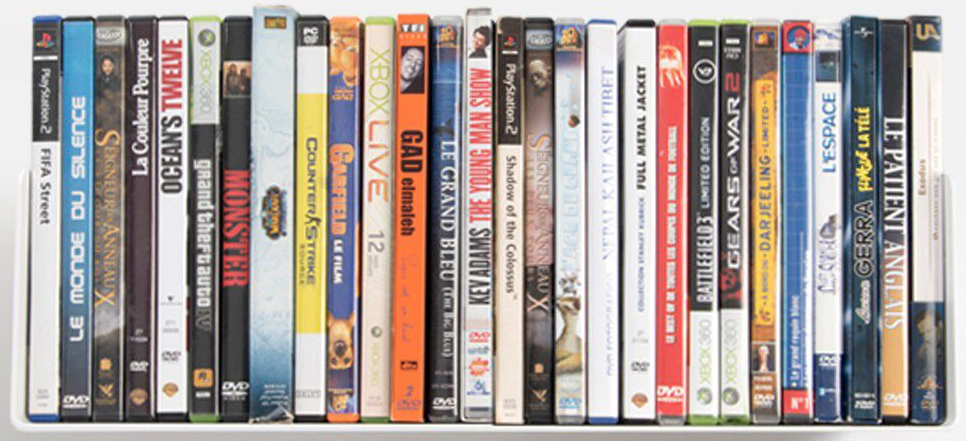
\includegraphics[width=\textwidth,height=3cm,keepaspectratio]{images/find_my_disk.png}
	\end{center}

	\item \textbf{Object manipulation:} All manipulation will be performed by the human operator under the supervision of the robot.

	\item \textbf{Object description and dialogs:} The robot shall provide accurate visual descriptions of the discs in the shelf, and those that are presented to it until the desired object is found. The robot can also lead the interaction by asking relevant questions (e.g.~\textit{what's the cover color?} or \textit{what's the title/author?}), so it can look in the spines and covers as necessary.\\
	It is also acceptable (although not advised), to review each title one by one.

	\item \textbf{Clear area:} The robot may assume that the working area is clear, with no people around making loud noises.

	\item \textbf{Disks:} A \textit{disk} can be the encasing of any CD, DVD, BluRays, audio cassettes, LP, etc. These objects will not be available for training during setup days, although samples can be provided.

	\item \textbf{Data recording:} The provided data must include:
	\begin{enumerate*}[label=(\roman*)]
		\item audio recording of the whole test,
		\item its transcript in plain text format,
		and
		\item a PDF summarizing the interaction.
	\end{enumerate*}
	The PDF report must contain:
	\begin{enumerate*}[label=(\alph*)]
		\item team name,
		\item the audio recording transcript,
		and
		\item each description provided backed with the source image.
	\end{enumerate*}

\end{enumerate}

\subsection{OC instructions}

\textbf{Setup days}
\begin{itemize}
	\item Provide media samples for practice.
\end{itemize}

\subsection{Referee instructions}
The referee needs to
\begin{itemize}
	\item Rearrange the disks on the bookcase.
	\item Provide instruction to the operator.
	\item Blindfold the operator.
\end{itemize}


% \newpage
\subsection{Score sheet}

The maximum time for this test is 5 minutes.

\begin{scorelist}
	\scoreheading{Main Goal}
	\scoreitem{1000}{Desired disk is found}

	\scoreheading{Bonus rewards}
	\scoreitem{500}{Provide labeled recorded data}
	\scoreitem{1000}{Help operator to find a second disk}

	% No longer necessary, computes automatically
	% \setTotalScore{1000}
\end{scorelist}


% Local Variables:
% TeX-master: "Rulebook"
% End:


% Local Variables:
% TeX-master: "Rulebook"
% End:

\newpage
\section{Hand Me That [Party Host]}
\label{test:hand-me-that}
A guest at the party speaks English, but with only a limited vocabulary. The robot will assist them in obtaining things that they gesture for.

%\subsection{Focus}
%Joint attention is a well-studied and important task in Human-Robot Interaction. The goal of this task is to really challenge the teams to perform a hard HRI task.

\subsection*{Main Goal}
The robot identifies (touching or naming) each object at which the operator is pointing at.

\noindent\textbf{Reward:} 2500pts (500pts per object)


% %% %%%%%%%%%%%%%%%%%%%%%%%%%%%%%%%%%%%%%%%%%%%%%%%%%%%%%%
%
% Setup
%
% %% %%%%%%%%%%%%%%%%%%%%%%%%%%%%%%%%%%%%%%%%%%%%%%%%%%%%%%
\subsection*{Setup}
\begin{enumerate}[nosep]
	\item \textbf{Location:} This takes place in a room in the arena.

	\item \textbf{Starting position:} The robot and the operator stand in a predefined location announced beforehand % (OC instructions: announce this 2 hours before the test).

	\item \textbf{Groups of Objects:} There are five groups of 2--5 objects randomly placed along the room

	\item \textbf{Deck:} The referee has a deck of objects to request, one per group, sorted by distance.

\end{enumerate}


% %% %%%%%%%%%%%%%%%%%%%%%%%%%%%%%%%%%%%%%%%%%%%%%%%%%%%%%%
%
% Procedure
%
% %% %%%%%%%%%%%%%%%%%%%%%%%%%%%%%%%%%%%%%%%%%%%%%%%%%%%%%%
\subsection*{Procedure}
\begin{enumerate}[nosep]
	\item \textbf{Pick an object} The robot asks the operator: \emph{what do you need?}. % We rule out natural language interaction
	Then
	\begin{enumerate}[nosep]
		\item The operator walks near to the object and points at it.
		\item The robot can asks as many questions as necessary.
		\item The operator replies to each question (most likely with \emph{yes}, \emph{no}, \emph{I don't know}, etc).
		\\\textbf{Remark:} The operator does not know the name of the object.
	\end{enumerate}
  \item \textbf{Repeat} Repeat up to 5 times for the maximum score.
\end{enumerate}


% %% %%%%%%%%%%%%%%%%%%%%%%%%%%%%%%%%%%%%%%%%%%%%%%%%%%%%%%
%
% Additional Rules
%
% %% %%%%%%%%%%%%%%%%%%%%%%%%%%%%%%%%%%%%%%%%%%%%%%%%%%%%%%
\subsection*{Additional rules and remarks}
\begin{enumerate}[nosep]
	\item \textbf{Keep going:} The robot should keep trying to determine the referred to object until they score or run out of time.

	\item \textbf{Skipping groups:} The robot may say \emph{Pass} or \emph{I give up} to try with the next object.

	\item \textbf{Incorrect guesses:} Incorrect guesses reduce the value of the correct guess by 200 points, each, the first two times. Guessing correctly on the third or fourth attempt is worth 100 points. After the fourth guess is worth no points.

	\item\textbf{Clarifying questions:} The robot is allowed to ask up to 3 clarifying questions per object. Each question applies a penalty of 150 points for that particular object. From 4 questions on, no points are awarded.

	\item\textbf{Uneducated operator:} The referee may instruct the operator to answer \emph{I don't understand} or \emph{I don't know} if the robot asks complex questions or is attempting blind guessing.

	\item \textbf{Groups of Objects:} A group consists of 2--5 random standard objects (see~\refsec{rule:scenario_objects}), separated one from another for about 2.5--10cm.
	The average distance between the starting position and each group ranges between 50cm and 150cm.

\end{enumerate}

\subsection*{Referee instructions}

The referee needs to
\begin{itemize}[nosep]
	\item Rearrange and mix groups between runs
	\item Verify that the operator is pointing at the right item
\end{itemize}

\subsection*{OC instructions}
During Setup days:
\begin{itemize}[nosep]
	\item Announce the starting position of the robot.
\end{itemize}


\subsection*{Score sheet}

The maximum time for this test is 10 minutes.

\begin{scorelist}
	% \scoreheading{Communicating}
	% \scoreitem[5]{500}{Correctly determine an item on the first attempt}
	% \penaltyitem[5]{-200}{Correctly determine an item on the second attempt}
	% \penaltyitem[5]{-400}{Correctly determine an item on the third or fourth attempt}
	% \penaltyitem[5]{-500}{Correctly determine an item on a subsequent attempt}
	% \penaltyitem[5]{-150}{Asking 1 clarifying question.}
	% \penaltyitem[5]{-300}{Asking 2 clarifying questions.}
	% \penaltyitem[5]{-450}{Asking 3 clarifying questions.}

	\scoreheading{Group 1}
	\scoreitem{500}{Name/touch the object being pointed}
	\penaltyitem[4]{-150}{Asking clarifying question}
	\penaltyitem[2]{-400}{Asking color/category question}
	\penaltyitem[2]{-200}{Incorrect guess}

	\vspace{-0.75\baselineskip}%
	\scoreheading{Group 2}
	\scoreitem{500}{Name/touch the object being pointed}
	\penaltyitem[4]{-150}{Asking clarifying question}
	\penaltyitem[2]{-400}{Asking color/category question}
	\penaltyitem[2]{-200}{Incorrect guess}

	\vspace{-0.75\baselineskip}%
	\scoreheading{Group 3}
	\scoreitem{500}{Name/touch the object being pointed}
	\penaltyitem[4]{-150}{Asking clarifying question}
	\penaltyitem[2]{-400}{Asking color/category question}
	\penaltyitem[2]{-200}{Incorrect guess}

	\vspace{-0.75\baselineskip}%
	\scoreheading{Group 4}
	\scoreitem{500}{Name/touch the object being pointed}
	\penaltyitem[4]{-150}{Asking clarifying question}
	\penaltyitem[2]{-400}{Asking color/category question}
	\penaltyitem[2]{-200}{Incorrect guess}

	\vspace{-0.75\baselineskip}%
	\scoreheading{Group 5}
	\scoreitem{500}{Name/touch the object being pointed}
	\penaltyitem[4]{-150}{Asking clarifying question}
	\penaltyitem[2]{-400}{Asking color/category question}
	\penaltyitem[2]{-200}{Incorrect guess}

	% No longer necessary, computes automatically
	% \setTotalScore{1000}
\end{scorelist}


% Local Variables:
% TeX-master: "Rulebook"
% End:


% Local Variables:
% TeX-master: "Rulebook"
% End:

\newpage
\section{Set the Table [Housekeeper]}
\label{test:set-the-table}
The robot has to set the table (presumably for dinner) for one person.

% \subsection*{Focus}
% This test focuses on object perception, manipulation, and planning.

\subsection*{Main Goal}
Neatly lay tableware and cutlery on the dining table (5 objects).

\noindent\textbf{Reward:} 1000pts

\subsection*{Bonus rewards}
\begin{enumerate}[nosep]
	\item Opening the cupboard drawer (250pts)
	\item Picking all utensils from the cupboard drawer (100pts each, max 500pts)
	\item Closing the cupboard drawer (100pts)
	\item Laying a place mat first (150pts)
	% \item Leaving the arena (100pts)
\end{enumerate}

\subsection*{Setup}
\begin{itemize}[nosep]
	\item \textbf{Location:} This test takes place in the arena, in a table close to the cupboard.
	\item \textbf{Table:} Chairs may be placed around the table and won't be removed.
	\item \textbf{Cupboard:} The cupboard doors and drawers are initially closed.
	\item \textbf{Objects:} The objects used in this test can be found in the cupboard, not in their predefined locations.
\end{itemize}


\subsection*{Additional rules and remarks}
\begin{enumerate}[nosep]
	\item \textbf{Deus ex Machina:} The following reductions apply:
	\begin{itemize}[nosep]
		\item \textbf{Handover:} Handing over an object causes a score reduction of 100pts.
		\item \textbf{Showing objects:} Pointing, or telling to the robot where an object is or where to place it causes a score reduction of 50pts.
		\item \textbf{Placing tableware:} Having a human assistant placing tableware on the table causes a score reduction of 200pts.
		\item \textbf{Placing cutlery:} Having a human assistant placing cutlery on the table causes a score reduction of 250pts.
	\end{itemize}

	\item \textbf{Table setup:} Knife and spoon go on the right of the dish with the mug or cup in front of them; fork and napkin go on the left side; and the bowl is stacked on top of the dish.

	The following distribution is used:
	\begin{itemize}[nosep]
		\item\textit{Silverware}: Any two different objects (fork, knife, or spoon).
		\item\textit{Tableware}: A dish and any other object (bowl, cup, or mug).
		\item\textit{Napkin}: A cloth or paper napkin.
	\end{itemize}


	\item \textbf{Safe placing:} Objects must be placed with care. It must be clear that the robot is trying to place the object, not throwing or dropping it.

	\item \textbf{Cupboard drawers:} The team decides whether the objects are inside one of the cupboard drawers (and which) or placed on the cupboard.
	When no drawers are available, objects can be placed inside the cupboard. The cupboard door is used instead.

\end{enumerate}

\subsection*{Referee instructions}

The referee needs to
\begin{itemize}
	\item Remove all objects from the table
	\item Place objects in the right place as requested by team (in the drawer or on the cupboard)
	\item Close all open doors and drawers
\end{itemize}

\subsection*{OC instructions}
During Setup days:
\begin{itemize}
	\item Provide official cutlery and tableware for training.
	\item Announce the default location of the cutlery and tableware on the cupboard.
\end{itemize}

% 2 hours before the test:
% \begin{itemize}
% 	\item Announce the predefined location to take the command.
% \end{itemize}

% \newpage
\subsection*{Score sheet}
The maximum time for this test is 10 minutes.

\begin{scorelist}
	\scoreheading{Main Goal}
	\scoreitem{1000}{Neatly arrange tableware and cutlery on the table (5 objects)}
	\penaltyitem[5]{50}{Pointing at object}
	\penaltyitem[5]{100}{Handover an object}
	\penaltyitem[5]{200}{Bypassing placement}

	\scoreheading{Bonus rewards}
	\scoreitem{250}{Opening the cupboard drawer door}
	\scoreitem[5]{100}{Picking an utensil from the cupboard drawer}
	\scoreitem{100}{Closing the cupboard drawer}
	\scoreitem{150}{Laying a place mat first}

	%\setTotalScore{1000}
\end{scorelist}


% Local Variables:
% TeX-master: "Rulebook"
% End:


% Local Variables:
% TeX-master: "Rulebook"
% End:


\newpage
\section{Stickler for the Rules (aka RoboCop) [Party Host]}
\label{test:stickler-for-the-rules}
The robot has to enforce house rules set by the homeowner.


\subsection*{Main Goal}
Identify all party guests breaking the house rules and politely ask them to stop.

\noindent\textbf{Reward:} 750pts (250pts per offender).

\subsection*{Bonus rewards}
\begin{enumerate}[nosep]
	\item Remind offenders the house rules and confirm obedience (750pts, 250pts each).
\end{enumerate}

\subsection*{Setup}
\begin{itemize}[nosep]
	\item \textbf{Location:} This test takes place in the arena.
	\item \textbf{Guests:} There are at least 5 party guests inside the arena.
\end{itemize}


\subsection*{House Rules:}
\begin{enumerate}[nosep]
	\item \textbf{Partial scoring:} The main task allows partial (per offender) scoring.
% \begin{enumerate}[nosep,label=\Roman.~]
	\item \textit{No shoes inside the house.}\\
	\textbf{Policy:} All guests have to take off their shoes at the entrance.\\
	\textbf{Action:} Take the guest to the entrance and verify she takes off her shoes.

	\item \textit{Black Room entrance forbidden}\\
	\textbf{Policy:} No guests are allowed in the \emph{Black Room}.
	\textbf{Action:} Take the offender with other party guests and verify she doesn't enter back.

	\item \textit{No littering}\\
	\textbf{Policy:} Guests are not allowed to leave garbage on the floor.
	\textbf{Action:} Make the (closest) offender to pick up the garbage and throw it into the bin.

	\item \textit{Compulsory hydration}\\
	\textbf{Policy:} All guests must have a drink in hand at all times.\\
	\textbf{Action:} Take the guest to the kitchen/bar and make sure she grabs a drink.
\end{enumerate}

\subsection*{Additional rules and remarks}
\begin{enumerate}[nosep]
	\item \textbf{Offenders:} Three of the guests are breaking rules.
	Offenders may not follow the robot's instructions.

	\item \textbf{Confirm law enforcement:} To get the bonus rewards the robot has to state when a guest did or did not follow the given instructions.

\end{enumerate}


\subsection*{Referee instructions}

The referee needs to
\begin{itemize}
	\item Instruct party guests on which rules to break.
	\item Assign each party guest a drink
\end{itemize}

\subsection*{OC instructions}
During Setup days:
\begin{itemize}
	\item Announce which room is the \textit{Black Room}.
\end{itemize}

\subsection*{Score sheet}

The maximum time for this test is 10 minutes.

\begin{scorelist}
	\scoreheading{Main Goal}
	\scoreitem[3]{250}{Recognize guests breaking rules and ask them to stop}
	\scoreheading{Bonus Goal}
	\scoreitem[3]{250}{Control if guests stop breaking rules}
\end{scorelist}


% Local Variables:
% TeX-master: "Rulebook"
% End:


% Local Variables:
% TeX-master: "Rulebook"
% End:





\chapter{Finals}

The competition ends with the Finals on the last day, where the four teams with the highest total score compete.
The \iterm{Finals} are conducted as a final open demonstration.
This demonstration does not have to be different from the Open Challenge. 
It does not have to be the same either.

To avoid logistical issues during the last day of the competition, the \iterm{Finals} are divided into two sets of demonstrations: the Bronze Competition and the RoboCup @Home Grand Finale.
The Bronze Competition is a set of demonstrations that are carried out before the RoboCup @home Grand Finale. Here, all the leagues run in parallel, with the fourth and third highest scored teams competing for the bronze.
Finally, the two teams with the highest score in each League present their demonstrations in a serialized manner during the RoboCup @Home Grand Finale.

Even though each league has its own first, second and third place, the RoboCup @Home Grand Finale is meant to show the best of all leagues to the jury members as well as the audience and, thus, warrants a single schedule slot.

\section{Evaluating Juries for Final Demonstrations}
\label{final:jury}
Each set of final demonstrations is evaluated by a different combination of evaluating juries, here described.

\begin{enumerate}
\item\textbf{League-internal jury:} The league-internal jury is formed by the Executive Committee.
The evaluation of the league-internal jury is based on the following criteria:
  \begin{compactenum}
  \item Scientific contribution %(maybe taken from the OC)
  \item Contribution to @Home %(evaluated by Execs/TC)
  \item Relevance for @Home / Novelty of approaches %(evaluated by execs/TC)
  \item Presentation and performance in the finals.
  \end{compactenum}

\item \textbf{League-external jury:} The league-external jury consists of people not being involved in the RoboCup@Home league,
but having a related background (not necessarily robotics).
They are appointed by the Executive Committee.
The evaluation of the league-external jury is based on the following criteria:
  \begin{compactenum}
  \item Originality and Presentation
    (story-telling is to be rewarded)
  \item Usability / Human-robot interaction
  \item Multi-modality / System integration
  \item Difficulty and success of the performance
  \item Relevance / Usefulness for daily life
  \end{compactenum}

\item\textbf{Teams-based jury:} The teams-based jury is formed by members of the league's teams.
The evaluation of the teams-based jury is based on the following criteria:
  \begin{compactenum}
  \item Scientific contribution %(maybe taken from the OC)
  \item Contribution to @Home %(evaluated by Execs/TC)
  \item Relevance for @Home / Novelty of approaches %(evaluated by execs/TC)
  \item Presentation and performance in the finals.
  \end{compactenum}
\end{enumerate}


\section{Bronze Competition (4th and 3rd Highest Scoring Teams)}
The demonstration is evaluated by one member of the league-internal jury, by one member of the league-external jury and by the complete team-based jury.
The final score and ranking are determined by the jury evaluations and by the previous performance (in Stages I and II) of the team, in the following manner:

\begin{enumerate}
  \item The influence of the league-internal jury member to the final ranking is \SI{15}{\percent}.
  \item The influence of the league-external jury member to the final ranking is \SI{15}{\percent}.
  \item The influence of the teams-based jury to the final ranking is \SI{15}{\percent}.
  \item The influence of the total sum of points scored by the team in Stage I and II is \SI{55}{\percent}.
\end{enumerate}

These demonstrations are carried out in parallel, having each League perform their own Bronze Competition in their own arena at the same time to save time.

\section{RoboCup@Home Grand Finale (2nd and 1st Highest Scoring Teams)}
The demonstration is evaluated by the complete league-internal and the complete league-external jury.
The final score and ranking are determined by the jury evaluations and by the previous performance (in Stages I and II) of the team, in the following manner:
  
\begin{enumerate}
  \item The influence of the league-internal jury to the final ranking is \SI{25}{\percent}.
  \item The influence of the league-external jury to the final ranking is \SI{25}{\percent}.
  \item The influence of the total sum of points scored by the team in Stage I and II is \SI{50}{\percent}.
\end{enumerate}

These demonstrations are carried out in a serialized fashion, one League performing after another in one arena.


\section{Common Description of Final Demonstrations}
Teams can choose freely what to demonstrate, however it is expected that teams present the scientific and technical contributions they submitted in both \iterm{team description paper} and the \iterm{RoboCup\char64Home Wiki}.
In addition, teams may provide a printed document to the jury (max 2 pages) that summarizes the demonstrated robot capabilities and contributions.  

\subsection{Task}
The procedure for the demonstration and the timing of slots is as follows:
\OpenDemonstrationTask{ten}{five}

\OpenDemonstrationChanges

%% %%%%%%%%%%%%%%%%%%%%%%%%
\section{Final Ranking and Winner}

The winner of the competition is the team that gets the highest
ranking in the finals.

There will be an award for 1st, 2nd and 3rd place. All teams in the
Finals receive a certificate stating that they made it into the Finals
of the RoboCup@Home competition.


% Local Variables:
% TeX-master: "Rulebook"
% End:



\printabx
\printidx

\end{document}
